\chapter{Powder Chemistry Effects on the Sintering Behavior of MgO-doped Bayer Alumina}

\section{Introduction}
Most commercial alumina products use Bayer processed powder because it is a lower cost option for products with purity levels of up to 99.9\%. The remaining 0.1\% consists of the intentionally added MgO dopant, and impurities such as Na$_{2}$O, CaO, Fe$_{2}$O$_{3}$, and SiO$_{2}$ that originate from the bauxite ore or the Bayer process itself. It is well known that trace (ppm) amounts of dopants or impurities can have a significant influence on the sintering of alumina \cite{Bae1994,Bae1997,Bae1993}. Since Coble's discovery of MgO doping to produce high-density translucent alumina, there has been high academic and commercial interest in understanding how small concentrations of dopants and impurities characteristic of Bayer alumina affect sintering \cite{Bennison1990,Jorgensen1965,Heuer1979,Louet2005a,Park2000a}.

In chapter 2, the influence of Na$_{2}$O and SiO$_{2}$ on the sintering of MgO-free Bayer alumina was investigated. Na$_{2}$O was shown to initially retard the densification of MgO-free Bayer alumina samples, but no effect was observed after extended sintering time (> 30 min) at 1525$^{\circ}$C, whereas the addition of SiO$_{2}$ to MgO-free Bayer alumina formed a liquid phase and significantly retarded densification throughout the entire sintering process. Na$_{2}$O addition to SiO$_{2}$-doped samples increased the densification rate and degree of densification compared to singly SiO$_{2}$-doped samples. Based on phase equilibria, the solubility of Al$_{2}$O$_{3}$ in the liquid phase was shown to increase as the Na$_{2}$O concentration in the liquid grain boundary phase increases. Furthermore, a higher Na$_{2}$O concentration decreases the viscosity of the liquid phase, which further increases the densification rate \cite{Frueh2016a}. Hence, samples with high Na$_{2}$O/SiO$_{2}$ ratios ($\geq$0.5) have higher densities than samples with lower Na$_{2}$O/SiO$_{2}$ ratios. 

MgO is commonly added to commercial alumina powders because it is known to improve sintering. Several reasonable mechanistic explanations for the beneficial effect of MgO include solute-drag, particle-pinning, modification of defect chemistry, increase of surface diffusivity, modification of a liquid phase, and modification of interfacial properties \cite{Bae1994}. A model that takes into account the redistribution of MgO and SiO$_{2}$ during the sintering of high purity alumina was reported by Handwerker et al. \cite{Handwerker1989} They proposed that MgO changes the segregation behavior of glass forming impurities such as SiO$_{2}$ by increasing their solubility in Al$_{2}$O$_{3}$. This mechanism was supported by the work of Gavrilov et al. \cite{Gavrilov1999} who demonstrated by high resolution secondary ion mass spectrometry that the dopants segregate strongly to grain boundaries when high purity Al$_{2}$O$_{3}$ is singly doped with either SiO$_{2}$ or MgO, but show a higher solubility in Al$_{2}$O$_{3}$ when co-doped with MgO and SiO$_{2}$ due to a defect mechanism in which Mg$^{2+}$ and Si$^{4+}$ occupy Al$^{3+}$ sites and compensate for each other's charge and strain. This model is of particular interest since it considers the direct interaction of MgO and SiO$_{2}$; an impurity known to negatively affect alumina densification. 

In this chapter it is reported how Na$_{2}$O and SiO$_{2}$ influence the sintering of 99.8 - 99.9\% pure Bayer alumina doped with 380 ppm MgO. Dilatometry and sintering kinetics of MgO-free Bayer alumina samples with similar Na$_{2}$O and SiO$_{2}$ concentrations from chapter 2 are compared to the present results to identify the stages at which MgO affects densification, and to identify key mechanisms that are responsible for the beneficial effect of MgO on the sintering of Bayer alumina. High-resolution transmission electron microscopy (TEM) and energy dispersive spectroscopy (EDS) measurements show the distribution of dopants/impurities on grain boundaries. First-principles calculations based on the density functional theory (DFT) were carried out to estimate the relative thermodynamic stability of MgO, SiO$_{2}$, and MgO+SiO$_{2}$ in the alumina lattice.


\section{Experimental}

A chemically purified MgO-doped Bayer alumina powder (Almatis, Inc., Leetsdale, PA, USA) was chosen for this study. Earlier we studied the influence of SiO$_{2}$ and Na$_{2}$O on the sintering of MgO-free Bayer alumina using a powder with similar physical and chemical characteristics as the powder used in this study. Since the sample preparation procedures of the two powders were identical, the differences in sintering behavior after doping with similar Na$_{2}$O and SiO$_{2}$ concentrations should be attributable primarily to the difference in MgO concentration and its cross effects with Na$_{2}$O and SiO$_{2}$. 

Physical and chemical characteristics of the powder are shown in Table \ref{Ch3-table:table1} and Figure \ref{Ch3-figure:Figure1}. The powder was doped with up to 1000 ppm Na$_{2}$O and 500 ppm SiO$_{2}$ using sodium acetate (NaC$_{2}$H$_{3}$O$_{2}$$\cdot$3H$_{2}$O, ACS grade, BDH, VWR International LLC, West Chester, PA, USA) and tetraethyl orthosilicate (Si(OC$_{2}$H$_{5}$)$_{4}$), 98\%, Aldrich Chemical Company, Inc. Milwaukee, WI, USA), respectively, to obtain chemistries similar to commercial high purity Bayer aluminas with different liquid volume fractions and different Na$_{2}$O/SiO$_{2}$ ratios, as shown in Table \ref{Ch3-table:table2}. The amount of liquid in the samples at 1525$^{\circ}$C was estimated from the Al$_{2}$O$_{3}$-Na$_{2}$O-SiO$_{2}$ and Al$_{2}$O$_{3}$-MgO-SiO$_{2}$ phase diagrams \cite{Frueh2016a,Mao2005,Lambotte2013a} based on the concentrations of SiO$_{2}$, Na$_{2}$O and MgO. The detailed doping procedures are described in chapter 2. 

Samples with green densities of 59.0 $\pm$ 0.5\% were fabricated for sintering studies by uniaxial and cold isostatic dry pressing (CIP, Autoclave engineers, Erie, Pa, USA) at 170 MPa and 200 MPa, respectively. The dry pressed cylinders were heated at 10$^{\circ}$C/min to 1525$^{\circ}$C in a thermomechanical analyzer (TMA, Linseis PT1600, Robbinsville, NJ, USA) to record the shrinkage during heating. The kinetics of sintering of samples at 1450$^{\circ}$C and 1525$^{\circ}$C were investigated for up to 8 h. The samples were heated at 10$^{\circ}$C/min to 1200$^{\circ}$C and then at 5$^{\circ}$C/min to the final sintering temperature. The average grain size and density were measured by the linear intercept (ASTM Standard E112-96) \cite{Standard2013} and Archimedes methods (ASTM standard B962-15) \cite{Standard2015}, respectively. The structure and chemistry of grain boundaries were investigated by transmission electron microscopy (TEM) and energy dispersive x-ray spectroscopy EDS using a dual aberration corrected FEI Titan$^{3}$ field emission microscope operated at 300 kV and FEI Talos (FEI, Hillsboro, OR, USA) field emission microscope at 200 kV. The EDS on both microscopes is an FEI Super-X system consisting of four SDDs (Silicon Drift Detectors) with a solid angle of 0.9 srad. The samples for TEM and EDS were air-quenched from the sintering temperature by pulling the samples out of the box furnace at temperature and prepared using a focused ion beam (Quanta 200 3D Dual Beam FIB, FEI, Hillsboro, OR, USA). Grain boundaries were chosen for analysis that were oriented parallel to the TEM beam in order to accurately measure grain boundary widths in the 2D projection images and EDS profiles. Chemical analyses were performed by inductively coupled plasma (ICP) emission spectroscopy (iCap 6000, Thermo Fischer Scientific, Inc., Waltham, MA, USA) after alumina samples were acid digested in a microwave digestion unit equipped with a Teflon$^{TM}$ sample holder (MARS M, CEM Corp., Matthews, NC, USA).

\section{Computational Methodology}

DFT-based first-principles calculations were carried out at 0 K to investigate the thermodynamic stability of clustered defects in the $\alpha$-alumina structure. The energy at 0 K without the contribution of the zero-point vibrational energy $E_{0}$ was obtained by an equation of state (EOS) fitting using the four-parameter Birch-Murnaghan (BM4) equation as follows \cite{Shang2010}:

%%
\begin{equation}
\label{Ch3-eq: EOS}
E_{0}(V) = a + bV^{- \frac{2}{3}} + cV^{- \frac{4}{3}} + dV^{-2}
\end{equation}
%%

\noindent where $a$, $b$, $c$, and $d$ are fitting parameters. The EOS fitting is achieved through an energy-volume (E-V) curve of at least 5 different volumes based on the methodology discussed by Shang et al. \cite{Shang2010}. The Helmholtz energy $F(V,T)$ can be predicted as a function of temperature $T$ and volume $V$ via \cite{Shang2010,Wang2004}:

%%
\begin{equation}
\label{Ch3-eq: helmholtz}
F(V,T) = E_{0}(V) + F_{vib}(V,T) + F_{T-el}(V,T)
\end{equation}
%%

\noindent where $F_{vib}$ is the temperature-dependent vibrational contribution, and $F_{T-el}$ is the thermal electronic contribution. At ambient pressure, the Helmholtz energy of the system is equal to the Gibbs energy. 

The vibrational contribution was obtained using the Debye-Gr\"uneisen model \cite{Shang2010}:

%%
\begin{equation}
\label{Ch3-eq: Fvib}
F_{vib}(V,T) = \frac{9}{8} k_{B} \theta_{D}(V) - k_{B}T \left [D\left( \frac{\theta_{D} (V)}{T} \right) + 3 ln \left(1-e^{-\theta_{D}(V)/T} \right) \right]
\end{equation}
%%

\noindent where $\theta_{D}$ is the Debye temperature, $T$ the temperature, and D[$\theta_{D}$(V)/T] the Debye function. The Debye temperature can be calculated by: 

%%
\begin{equation}
\label{Ch3-eq: debyetT}
\theta_{D} = s \frac{(6\pi^{2})^{\frac{1}{3} \hbar}}{k_{B}} V_{0}^{\frac{1}{6}} \left(\frac{B_{0}}{M} \right)^{\frac{1}{2}} \left(\frac{V_{0}}{V} \right)^{\gamma}
\end{equation}
%%

\noindent where $s$ is the Debye temperature scaling factor, $\gamma$ the Gr\"uneisen parameter determined by the pressure derivative of bulk modulus $B'$, $B_{0}$ the equilibrium bulk modulus, $M$ the atomic mass, and $V_{0}$ the equilibrium volume. Here, the equilibrium properties $V_{0}$, $B_{0}$, and $B'$ are estimated from the EOS of Eq. \ref{Ch3-eq: EOS}. The methodology by Liu et al. \cite{Liu2015} was used to calculate the scaling factor of Al$_{2}$O$_{3}$: 

%%
\begin{equation}
\label{Ch3-eq: scalingfactor}
s(\nu) = 3^{\frac{5}{6}} \left( 4 \sqrt{2} \left(\frac{1+\nu}{1-\nu}\right)^{\frac{3}{2}} + \left(\frac{1+\nu}{1-\nu}\right)^{\frac{3}{2}}\right)^{-\frac{1}{3}}
\end{equation}
%%

\noindent where $\nu$ is the Poisson's ratio, which was calculated by Shang et al. \cite{Shang2007c}. The thermal electronic contribution was estimated based on the electronic density of states and the Fermi-Dirac statistics \cite{Wang2004}.

In the present work, the Vienna Ab-initio Simulation Package (VASP) was used to perform the first-principles calculations \cite{Kresse1996}. The projector augmented-wave (PAW) \cite{Kresse1999,Blochl1994} method was utilized to describe the electron-ion interactions with the exchange correlation functional given by the generalized gradient approximation (GGA-PW91) \cite{Perdew1992}. A sigma value of 0.2 eV and a plane wave energy cutoff of 1.3 times higher than the highest default cutoff were adopted, which was 520 eV. The Brillouin zone sampling was carried out with Bl\"ochl corrections using a gamma centered Monkhorst-Pack (MP) scheme \cite{Blochl1994,Monkhorst1976a}. The automated k-points grid generator in VASP was employed with a subdivision length of 80. The k-points generated by VASP for these calculations was 19x19x6. The energy convergence criterion of the electronic self-consistency was set at 10$^{-5}$ eV/atom for all calculations.

The energies of charge, site, and mass balanced defects in $\alpha$-alumina were calculated for defect clusters, i.e. the defects are located next to each other, since this has been shown to be the most stable configuration \cite{Atkinson2003}. The geometric arrangements of each of the clusters were chosen based on previous computational work. Multiple authors showed that a 30-40 atom supercell of Al$_{2}$O$_{3}$ is sufficient to calculate non-charged defects \cite{Atkinson2003,Grimes1994,Lagerlof1998,Xiang2015,Sarsam2013}. Multiple authors have studied charged and clustered defects in Al$_{2}$O$_{3}$ \cite{Atkinson2003,Grimes1994,Lagerlof1998,Xiang2015,Sarsam2013}. They showed that different geometric arrangements and supercell size result in little difference in energy and that the impurity atoms prefer to be clustered due to the binding energy \cite{Atkinson2003,Grimes1994,Lagerlof1998,Xiang2015,Sarsam2013}. Using this methodology, supercells were generated in the present work with Mg and/or Si clustered, i.e. the Mg-cluster having two Mg atoms substituted for two Al atoms and an oxygen vacancy as nearest neighbors, the Si-cluster having three Si atoms substituted for three Al atoms and an Al vacancy, and the Mg+Si-cluster having one Mg and one Si substituted for two Al atoms. 

\section{Sintering and Microstructure Analysis}

In chapter 2, it was shown that a glass phase can form during sintering of Bayer alumina. Table \ref{Ch3-table:table2} shows the amounts of liquid in the samples at 1525$^{\circ}$C estimated from the Al$_{2}$O$_{3}$-Na$_{2}$O-SiO$_{2}$ and Al$_{2}$O$_{3}$-MgO-SiO$_{2}$ phase diagrams based on the amount of SiO$_{2}$, Na$_{2}$O and MgO \cite{Mao2005}. It should be noted that it was proposed in the literature \cite{Subramaniam2006} that the composition of the glass in grain boundaries can deviate from the bulk glass composition predicted from the phase diagram. Therefore, the estimations from the phase diagram are approximations. It can be seen that the glass volume fraction increases from 0.03 vol.\% for SiO$_{2}$ concentrations of 82 ppm to 0.21 vol.\% for SiO$_{2}$ concentrations of 582 ppm at 1525$^{\circ}$C. 

Figure \ref{Ch3-figure:Figure2} shows the dilatometry curves of MgO-doped and MgO-free samples with different Na$_{2}$O and SiO$_{2}$ concentrations heated at 10$^{\circ}$C/min to 1525$^{\circ}$C. For samples with SiO$_{2}$ concentrations of 582 ppm the estimated amount of liquid increases from 0.18 vol.\% to 0.21 vol.\% during heating from 1250$^{\circ}$C to 1525$^{\circ}$C, and for samples with 82 ppm SiO$_{2}$ the amount of liquid phase is estimated from the phase diagram to increase from 0.026 vol.\% to 0.030 vol.\% during heating from 1250$^{\circ}$C to 1525$^{\circ}$C. 

Figure \ref{Ch3-figure:Figure2}a shows that the onset of densification (taken as the temperature at which the sample shrinkage is 0.1\%) of MgO-doped specialty alumina is shifted from $\sim$1050$^{\circ}$C for samples with 60 ppm Na$_{2}$O to $\sim$1100$^{\circ}$C for samples with 560 ppm Na$_{2}$O. Samples with 560 ppm Na$_{2}$O shrink 1\% less than samples with 60 ppm Na$_{2}$O after heating to 1525$^{\circ}$C. In both the MgO-doped and the MgO-free powders, higher SiO$_{2}$ concentrations retard densification at $\sim$1250$^{\circ}$C. However, the retardation caused by higher SiO$_{2}$ concentrations is less severe in the MgO-doped powder than in the MgO-free powder; e.g. already at 1300$^{\circ}$C, MgO-doped powder samples with 582 ppm SiO$_{2}$ (after the addition of 500 ppm SiO$_{2}$) shrink 0.2\% less and are 0.5\% less dense than samples with 82 ppm SiO$_{2}$, whereas samples of the MgO-free powder with 603 ppm SiO$_{2}$ shrink 0.5\% less and are 3.2\% less dense than samples with 103 ppm SiO$_{2}$. After reaching 1525$^{\circ}$C the dilatometry curves show that MgO-doped samples with 582 ppm SiO$_{2}$ (0.21 vol.\% glass) shrink 1.8\% less and are 5.4\% less dense than MgO-doped samples with 82 ppm SiO$_{2}$ (0.03 vol.\% glass). In contrast, the retardation of densification caused by the addition of 500 ppm SiO$_{2}$ to the MgO-free powder results in 3.0\% less linear shrinkage and 8.7\% lower relative densities after heating to 1525$^{\circ}$C. MgO-doped (380 ppm) powder samples with 560 ppm Na$_{2}$O and 582 ppm SiO$_{2}$ shrink $\sim$2.5\% less than samples with 60 ppm Na$_{2}$O and 82 ppm SiO$_{2}$ after reaching 1525$^{\circ}$C, and MgO-free powder samples with 529 ppm Na$_{2}$O and 603 ppm SiO$_{2}$ shrink $\sim$3.0\% less than samples with 29 ppm Na$_{2}$O and 103 ppm SiO$_{2}$ after reaching 1525$^{\circ}$C.

Figure \ref{Ch3-figure:Figure3}a and b show how the sintering kinetics of MgO-doped and MgO-free alumina are affected by Na$_{2}$O and SiO$_{2}$ after heating at 1450$^{\circ}$C and 1525$^{\circ}$C for up to 8 h. The density of samples with higher SiO$_{2}$ concentrations, i.e. higher glass concentrations, is lower for all hold times at 1450$^{\circ}$C and 1525$^{\circ}$C. At 1450$^{\circ}$C MgO-doped powder samples with 0.19 vol.\% glass phase (582 ppm SiO$_{2}$) are 6-7\% less dense than samples with 0.027 vol.\% glass phase (82 ppm SiO$_{2}$), for all hold times (Figure \ref{Ch3-figure:Figure3}a). At 1525$^{\circ}$C MgO-doped powder samples with 0.21 vol.\% glass phase are $\sim$11\% and $\sim$2\% less dense than samples with 0.03 vol.\% glass phase after heating for 0 h and 8 h, respectively, and samples with 0.03 vol.\% glass phase reach densities >98\% after 1 h, whereas samples with 0.066 and 0.21 vol.\% glass phase are only $\sim$96\% and $\sim$94\% dense, respectively (Figure \ref{Ch3-figure:Figure3}b). 

The effect of Na$_{2}$O concentration on densification strongly depends on glass phase concentration. In all samples a higher Na$_{2}$O concentration initially retards densification. For example, after 0 h at 1450$^{\circ}$C the relative density of samples with 0.03 vol.\% glass phase and 560 ppm Na$_{2}$O is $\sim$3\% lower than the relative density of samples containing the same amount of glass phase and 60 ppm Na$_{2}$O.  However, there is no difference in sintered density after 3 h at either 1450$^{\circ}$C or 1525$^{\circ}$C. For samples with higher glass phase concentrations (e.g., 0.21 vol.\%) the effect of Na$_{2}$O on the densification is more complicated, due to the changing Na$_{2}$O/SiO$_{2}$ ratio from 0.1 to 0.9 (Table \ref{Ch3-table:table2}). Samples with 0.21 vol.\% glass phase and Na$_{2}$O/SiO$_{2}$ ratios of 0.9 are 1-2\% denser than samples with 0.21 vol.\% glass phase and Na$_{2}$O/SiO$_{2}$ ratios of 0.1. However, after 30 min at 1525$^{\circ}$C the relative density of samples with 0.21 vol.\% glass phase and Na$_{2}$O/SiO$_{2}$ ratios of 0.9 in the glass phase is 0.9\% lower than the relative density of samples with 0.21 vol.\% glass phase and Na$_{2}$O/SiO$_{2}$ ratios of 0.1 in the glass phase, and after 1 h or longer at 1525$^{\circ}$C there is no difference in relative density. Samples with 0.066 vol.\% glass phase are 98.3 - 98.6\% dense after 8 h at 1525$^{\circ}$C, and samples with 0.21 vol.\% glass phase are 97.1\% - 97.5\% dense after 8 h at 1525$^{\circ}$C. 

Comparing the as-received MgO-free and MgO-doped powders with 0.03 vol.\% glass phase shows that doping with 380 ppm MgO leads to 1\% higher densities for all hold times at 1525$^{\circ}$C (Figure \ref{Ch3-figure:Figure3}b and c). After 8 h at 1525$^{\circ}$C the MgO-doped samples with 0.21 vol.\% glass phase are $\sim$2\% less dense than samples with 0.03 vol.\% glass phase, whereas the addition of 500 ppm SiO$_{2}$ (total of 603 ppm SiO$_{2}$ and 0.22 vol.\% glass) to the MgO-free powder leads to $\sim$4\% less dense samples. MgO-free and MgO-doped Bayer alumina samples containing 0.22 and 0.21 vol.\% glass phase, respectively, and global Na$_{2}$O/SiO$_{2}$ ratios of 0.9 show initial retardation of densification compared to samples with Na$_{2}$O/SiO$_{2}$ ratios of 0.1, but have higher densities than samples with Na$_{2}$O/SiO$_{2}$ ratios of 0.1 after further heating. This increased densification can be explained by the increased solubility of Al$_{2}$O$_{3}$ into the liquid grain boundary phase and the higher diffusivity (lower viscosity of the grain boundary phase) as the Na$_{2}$O/SiO$_{2}$ ratio increases \cite{Frueh2016a,Kwon1991}. However, after hold times of 1 h or longer at 1525$^{\circ}$C, MgO-free powder samples with 0.22 vol.\% glass phase and Na$_{2}$O/SiO$_{2}$ ratios of 0.9 are 1\% denser than samples with 0.22 vol.\% glass phase and Na$_{2}$O/SiO$_{2}$ ratios of 0.1, whereas MgO-doped powder samples with 0.21 vol.\% and Na$_{2}$O/SiO$_{2}$ ratios of 0.9 have the same densities as samples with 0.21 vol.\% glass phase and Na$_{2}$O/SiO$_{2}$ ratios of 0.1. 

The microstructures of samples with different vol.\% glass phase and different Na$_{2}$O/SiO$_{2}$ ratios heated at 1525$^{\circ}$C for 8 h are shown in Figure \ref{Ch3-figure:Figure4}. Samples with 60 ppm Na$_{2}$O show mostly equiaxed grains, regardless of the glass phase concentration in the samples (Figures \ref{Ch3-figure:Figure4}a and c). Samples with 560 ppm Na$_{2}$O (Figures  \ref{Ch3-figure:Figure4}b and d) show more facetted $\alpha$-Al$_{2}$O$_{3}$ grains and appear to have a wider grain size distribution than samples with 60 ppm Na$_{2}$O. These effects are more pronounced in samples with higher glass concentrations. The grain sizes of samples with 0.21 vol.\% glass are less than the grain sizes of samples with 0.03 vol.\% glass phase. 

The average grain sizes of samples with different vol.\% glass phase and different Na$_{2}$O/SiO$_{2}$ ratios are plotted as a function of relative density in Figure \ref{Ch3-figure:Figure5}. Grain growth starts when the final sintering stage is reached, between 85 and 92\% relative density. Samples with 0.03 vol.\% glass phase and 60 ppm Na$_{2}$O show a three-fold increase in grain size, from 0.5 $\mu$m to $\sim$1.5 $\mu$m, when the relative density increases from 68\% to 99\%, and samples with 0.03 vol.\% glass phase and 560 ppm Na$_{2}$O have a somewhat larger grain size of 2.2 $\mu$m at 99\% relative density. When relative densities of $\sim$99\% are reached in samples with 0.03 vol.\% glass, the grain size increases to 3.1 - 3.4 $\mu$m when heated at 1525$^{\circ}$C for 8 h. Samples with higher glass concentrations have a similar trajectory up to 92\% density. However, at densities >92\% the grain size of samples with higher glass phase concentrations increases stronger at lower densities compared to samples with lower densities. For example, 97.0-97.5\% dense samples with glass phase concentrations of 0.21 and 0.17 vol.\% have grain sizes of 2.6 and 2.4 $\mu$m, respectively, whereas samples with glass phase concentrations of 0.03 vol.\% have a grain size of 1.5 $\mu$m at the same relative density.
 
\section{Mechanistic Interpretation}

If the mechanism of MgO increasing the solubility of SiO$_{2}$ in alumina, as proposed by Handwerker et al. \cite{Handwerker1989}, is responsible for the improved sintering behavior of alumina, then the amount of liquid phase in MgO-doped alumina should be less than calculated and less than in MgO-free samples, and, the grain boundary thickness in MgO-doped alumina should be less than in MgO-free powder. The reduced grain boundary thickness in MgO-doped alumina should lead to a change in grain boundary chemistry and different sintering behavior after this co-dissolution has occurred compared to MgO-free alumina. 

Comparing the dilatometry curves and sintering kinetics of MgO-doped and MgO-free Bayer alumina powders with different chemistries shows that there are two stages at which MgO affects densification. At 1250$^{\circ}$C increased SiO$_{2}$ concentrations retard densification, and at the same stage there is an enhancement of densification due to MgO. This suggests that there is a direct interaction between SiO$_{2}$ and MgO at this stage, where MgO mitigates the negative effect of SiO$_{2}$. In ultrahigh purity alumina SiO$_{2}$ has been reported to decrease the concentration of Al interstitials and O vacancies, which decreases the diffusion rate during intermediate stage sintering (>1200$^{\circ}$C) \cite{Louet2008}. However, a liquid phase forms during the sintering of Bayer alumina at temperatures as low as 1200$^{\circ}$C due to the presence of other impurities and dopants such as Na$_{2}$O and MgO. Therefore, Bayer alumina densifies by liquid phase sintering. The Al$_{2}$O$_{3}$-SiO$_{2}$-MgO phase diagram suggests that MgO increases the solubility of Al$_{2}$O$_{3}$ in the liquid, and MgO can lower the viscosity of the glass melt \cite{Wu2015}, which results in higher diffusion coefficients. The enhanced diffusion associated with the lower viscosity and higher solubility of Al$_{2}$O$_{3}$ in the glass phase can explain why MgO positively affects the sintering of alumina at stages when SiO$_{2}$ would negatively affect densification. 

The second stage at which MgO affects densification is after 1 h at 1525$^{\circ}$C. MgO-free powder samples with 0.22 vol.\% glass phase and Na$_{2}$O/SiO$_{2}$ ratios of 0.9 have 1-2\% higher relative densities than samples with 0.22 vol.\% glass phase and Na$_{2}$O/SiO$_{2}$ ratios of 0.1 for all hold times at 1525$^{\circ}$C. In previous work we calculated an expected grain boundary thickness of 1.3 nm for samples with 0.22 vol.\% glass phase after 3 h at 1525$^{\circ}$C, based on the observed grain size of 1.6 $\mu$m assuming spherical monodispersed grains as an approximation.. The addition of 500 ppm Na$_{2}$O increases the Na$_{2}$O/SiO$_{2}$ ratio from 0.1 to 0.9, which modifies the liquid grain boundary phase and enhances densification as shown in Chapter 2. Figure \ref{Ch3-figure:Figure6} shows a high-resolution TEM image of a grain boundary of a MgO-free powder sample (2 ppm MgO) with 0.22 vol.\% glass phase and a Na$_{2}$O/SiO$_{2}$ ratio of 0.9 after 3 h at 1525$^{\circ}$C. It can be seen that the measured grain boundary thickness of 1.7 nm is close to the grain boundary thickness calculated based on the amount of glass phase in the sample. MgO-doped powder samples with 0.21 vol.\% glass phase and Na$_{2}$O/SiO$_{2}$ ratios of 0.9 have 1-2\% higher densities than samples with 0.21 vol.\% glass phase and Na$_{2}$O/SiO$_{2}$ ratios of 0.1 for most hold times at 1450$^{\circ}$C and for hold times < 30 min at 1525$^{\circ}$C. This difference in densification behavior is similar to the densification behavior of MgO-free powder samples, which suggests the presence of a liquid phase that is modified by Na$_{2}$O, as seen in the MgO-free alumina samples. 

Figure \ref{Ch3-figure:Figure7}a shows a high resolution TEM image of a grain boundary in an MgO-doped alumina sample with 0.21 vol.\% glass phase and a Na$_{2}$O/SiO$_{2}$ ratio of 0.9 after 0 h at 1525$^{\circ}$C. The measured grain boundary thickness of $\sim$1.4 nm for this sample is in agreement with the theoretically estimated \cite{Frueh2016a} grain boundary thickness. However, after 1 h or longer at 1525$^{\circ}$C, samples with 0.21 vol.\% glass and Na$_{2}$O/SiO$_{2}$ ratios of 0.9 have the same densities as samples with 0.21 vol.\% glass and Na$_{2}$O/SiO$_{2}$ ratios of 0.1, and the grain boundary thicknesses of those samples after 3 h at 1525$^{\circ}$C are $\sim$0.5 nm (Figure \ref{Ch3-figure:Figure7}b) and substantially thinner than the calculated grain boundary thickness of 1.4 nm.

The thinner grain boundary demonstrates that the addition of MgO causes a reduction of the amount of liquid phase in the grain boundaries after longer time at 1525$^{\circ}$C. In the literature it is reported that excess liquid phase, after an equilibrium grain boundary thickness \cite{Subramaniam2006} is reached, can accumulate in triple pockets. However, we did not observe any triple pockets in the 380 ppm MgO-doped samples with 0.21 vol.\% glass. Therefore, the impurities and dopants that formed the liquid phase after 0 h have to be distributed elsewhere in the sample after 3 h at 1525$^{\circ}$C. Since SiO$_{2}$-containing second phases, such as mullite or cordierite, were not observed in the samples, we hypothesize that SiO$_{2}$ and MgO form a solid solution in $\alpha$-alumina, as proposed by Handwerker et al. \cite{Handwerker1989}. This co-dissolution mechanism would significantly reduce the total amount of SiO$_{2}$ and, therefore, the liquid phase content in the samples and in the grain boundaries. 

The EDS maps in Figure \ref{Ch3-figure:Figure8} show the distribution of Si around a grain boundary in MgO-doped samples with a calculated glass concentration of 0.21 vol.\% after 0 h and 3 h at 1525$^{\circ}$C. Figure \ref{Ch3-figure:Figure9} shows the corresponding EDS line scans for Si and Mg across the grain boundaries. It can be seen that after 0 h at 1525$^{\circ}$C SiO$_{2}$ and MgO are strongly concentrated in the grain boundaries, and a chemical grain boundary thickness, $\delta_{chem}$, of $\sim$1.7 nm is estimated (Figures \ref{Ch3-figure:Figure8}a and \ref{Ch3-figure:Figure9}a), which is close to the structural grain boundary thickness of 1.4 nm measured from the high resolution TEM image (Figure \ref{Ch3-figure:Figure7}a). After 3 h at 1525$^{\circ}$C MgO and SiO$_{2}$ are still concentrated on the grain boundary, however, the chemical grain boundary thickness, $\delta_{chem}$, is $\sim$3.2 nm (Figure \ref{Ch3-figure:Figure8}b and \ref{Ch3-figure:Figure9}b) and substantially thicker than the observed structural grain boundary thickness, $\delta_{str}$, of $\sim$0.5 nm (Figure \ref{Ch3-figure:Figure7}b). This difference in structural and chemical grain boundary thickness after 3 h supports the argument that MgO and SiO$_{2}$ form a solid solution in the alumina lattice in the near grain boundary region. If we assume that equal amounts of MgO and SiO$_{2}$ dissolve into the alumina lattice to form the proposed defect complex, and that all MgO in the sample is consumed by this process, then 380 ppm SiO$_{2}$ must be removed from the amorphous grain boundary phase. This would leave 202 ppm SiO$_{2}$ in the grain boundaries to form the amorphous film with a calculated grain boundary thickness of 0.5 nm, which agrees with the observed grain boundary thickness of 0.5 nm.

To further evaluate whether MgO and SiO$_{2}$ form a solid solution in $\alpha$-alumina we conducted first-principles calculations based on density functional theory to gain insight into the thermodynamic stability of Mg$^{2+}$ and Si$^{4+}$ by themselves and together in the $\alpha$-alumina structure. To ensure the accuracy of the calculations, the lattice parameters and energy of the $\alpha$-alumina structure without any substitutions are compared with previous experiments and calculations in Table \ref{Ch3-table:table3}. It can be seen that the calculated lattice parameters match well with experimental values and lattice parameters from previous first-principles calculations \cite{Jain2013,MaterialsProject,Graham1960_595,Bergerhoff1983,Karlsruhe,Atkinson2003}. The difference between the present and past first-principles calculations can be attributed to the different input parameters used. 

We calculated the energy of a unit cell of the $\alpha$-alumina structure with substitutions according to the following balanced equations:\newline
\newline
\noindent Mg-Cluster: 
\begin{equation}
\label{Ch3-eq: Mgcluster}
2MgO + 2Al_{Al}^{x} + O_{O}^{x} \longrightarrow 2Mg_{Al}^{'} + V_{O}^{^{..}} + Al_{2}O_{3}
\end{equation}
%%
\newline
\noindent Si-Cluster:
\begin{equation}
\label{Ch3-eq: Sicluster}
3SiO_{2} + 4Al_{Al}^{x} \longrightarrow 3Si_{Al}^{^{.}} + V_{Al}^{'''} + 2Al_{2}O_{3}
\end{equation}
%%
\newline
\noindent Mg+Si-Cluster:
\begin{equation}
\label{Ch3-eq: MgSicluster}
MgO + SiO_{2} + 2Al_{Al}^{x} \longrightarrow Mg_{Al}^{'} + Si_{Al}^{^{.}} + Al_{2}O_{3}
\end{equation}
%%


\noindent Defect simulations of aliovalent cation substitutions in alumina \cite{Atkinson2003} showed that the dominant compensation mechanisms for Mg$^{2+}$ and Si$^{4+}$ by themselves in alumina are the formation of oxygen and aluminum vacancies, respectively (Eq. \ref{Ch3-eq: Mgcluster} and \ref{Ch3-eq: Sicluster}). In Eq. \ref{Ch3-eq: MgSicluster} Mg$^{2+}$ and Si$^{4+}$ compensate for each other's charge and the formation of vacancies or interstitials is unnecessary to account for dissolution in the alumina lattice. The calculations were carried out for clustered defects since they are lower in energy than isolated defects \cite{Atkinson2003}. The structures were relaxed and the formation energies as a function of temperature with bulk Al$_{2}$O$_{3}$ as the reference state are plotted in Figure \ref{Ch3-figure:Figure10}. It can be seen that the formation energy for the Mg+Si-cluster, $E_{Form}^{Mg+Si}$, is lower than the formation energies of the Mg-cluster, $E_{Form}^{Mg}$, and the Si-cluster, $E_{Form}^{Si}$, which shows that the Mg+Si-cluster is more stable than the Mg-cluster and the Si-cluster. Since two Mg$^{2+}$ ions and three Si$^{4+}$ ions are necessary to form the Mg-cluster and Si-cluster, respectively, but only one Mg$^{2+}$ and one Si$^{4+}$ are required to form the Mg+Si-cluster, the formation energies of the clusters can be compared by 

%%
\begin{equation}
\label{Ch3-eq: eform}
\bigtriangleup E_{Form}=E_{Form}^{Mg+Si} - \left( \frac{1}{3} E_{Form}^{Si} + \frac{1}{2}E_{Form}^{Mg} \right)
\end{equation}
%%

\noindent The formation energy difference, $\bigtriangleup E_{Form}$, is plotted in Figure \ref{Ch3-figure:Figure10} and it can be seen that $\bigtriangleup E_{Form}$ is negative at all temperatures, which means that the Mg+Si-cluster is more energetically favored to form than the Mg-cluster or Si-cluster. This shows that MgO and SiO$_{2}$ have a higher co-solubility in $\alpha$-alumina than MgO or SiO$_{2}$ by themselves. In $\alpha$-alumina the Al$^{3+}$ cation sites are 6-fold coordinated and Al$^{3+}$ has an effective ionic radius of 53.5 pm, while the radii of Mg$^{2+}$ and Si$^{4+}$ are 72 pm and 40 pm, respectively. Therefore, Mg$^{2+}$ and Si$^{4+}$ can compensate for each other's size and charge difference relative to Al$^{3+}$ in the $\alpha$-alumina lattice, which explains the lower energy of the Mg+Si-cluster. The stable phases for MgO and/or SiO$_{2}$ and Al$_{2}$O$_{3}$ are spinel, cordierite, and mullite. However, we hypothesize that if both MgO and SiO$_{2}$ are present at low concentrations, then it is more favorable for MgO and SiO$_{2}$ to form a solid solution in the $\alpha$-alumina structure than to form a second phase or remain in the grain boundaries as a siliceous liquid phase. 

The described mechanism could also influence the distribution of other oxides in the samples, such as Fe$_{2}$O$_{3}$, CaO, and Na$_{2}$O. Figure \ref{Ch3-figure:Figure11} shows the element distribution obtained from EDS of two grain boundaries in samples sintered at 1525$^{\circ}$C for 0 h and 3 h, respectively. Figures \ref{Ch3-figure:Figure11}a and e show the segregation of MgO to the grain boundaries after 0 h and 3 h, respectively, and it can be seen that after 0 h at 1525$^{\circ}$C Mg is more strongly concentrated in the grain boundary than after 3 h at 1525$^{\circ}$C, due to the mechanism described above. From Figures \ref{Ch3-figure:Figure11}b and f it can be seen that there is no segregation of Fe$_{2}$O$_{3}$, which indicates that Fe$_{2}$O$_{3}$ is in solid solution in the alumina lattice \cite{Atkinson2003}, since the Al$_{2}$O$_{3}$-Fe$_{2}$O$_{3}$ phase diagram shows considerable solubility \cite{Raghavan2010}. Figures \ref{Ch3-figure:Figure11}c, d, g, and h show that there is a slightly higher Na and Ca signal coming from the grain boundaries, showing that Na and Ca segregate to the grain boundaries and are components of the liquid grain boundary phase. Ca is more concentrated in the grain boundary after 3 h at 1525$^{\circ}$C, due to the narrower grain boundary thickness (Figure \ref{Ch3-figure:Figure7}b). 

It can be seen that the Na signal after 0 h at 1525$^{\circ}$C (Figure \ref{Ch3-figure:Figure11}c) shows a slight segregation of Na to the grain boundary, but after 3 h at 1525$^{\circ}$C (Figure \ref{Ch3-figure:Figure11}g) no segregation can be observed. It should also be noted that it is challenging to detect Na using EDS since the Na signal disappears quickly after the high-voltage electron beam is focused on the grain boundary. Therefore, we believe that there is still Na on the grain boundaries, even though the EDS map does not show an increased Na signal. However, since the Na signal is lower, we believe that after 3 h at 1525$^{\circ}$C there is less Na$_{2}$O on the grain boundaries than after 0 h at 1525$^{\circ}$C. The reduced amount of Na might be a result of volatilization of Na$_{2}$O during sintering. Figure \ref{Ch3-figure:Figure12} shows the influence of sintering time and temperature on the Na$_{2}$O concentration, obtained by ICP analysis, during sintering for samples with target concentrations of 560 ppm Na$_{2}$O. Between 1300$^{\circ}$C and 1525$^{\circ}$C the Na$_{2}$O concentration is constant at $\sim$510 ppm, which is 50 ppm below the target level. The lower Na$_{2}$O concentration might be due to volatilization at earlier stages. After heating to 1600$^{\circ}$C there is a loss of $\sim$250 ppm or a $\sim$50\% decrease in Na$_{2}$O concentration (Figure \ref{Ch3-figure:Figure12}a). After sintering at 1525$^{\circ}$C for 30 min the Na$_{2}$O concentration decreases by about 210 ppm or 40\%, but remains constant at $\sim$300 ppm when heated to 1525$^{\circ}$C for up to 8 h (Figure \ref{Ch3-figure:Figure12}b). This Na$_{2}$O loss between 0 and 30 min at 1525$^{\circ}$C can explain the lower Na signal in Figure \ref{Ch3-figure:Figure11}g. 

As explained earlier, the described dissolution of MgO and SiO$_{2}$ into the alumina lattice reduces the amount of glass phase in the grain boundaries. Since only SiO$_{2}$ is removed from the glass phase and other components of the glass phase, such as CaO and Na$_{2}$O remain, the grain boundaries can supersaturate. This can eventually lead to the nucleation of second phases, which was observed for samples with lower SiO$_{2}$ concentrations of 82 and 182 ppm.

\section{Summary and Conclusion}

The effect of MgO on the sintering of Bayer alumina powders with different chemistry was analyzed by comparing the sintering kinetics of MgO-free and MgO-doped Bayer aluminas with different impurity levels and ratios of Na$_{2}$O and SiO$_{2}$. TEM images of grain boundaries shows that the grain boundary thickness of MgO-doped Bayer alumina is reduced during densification at 1525$^{\circ}$C and are thinner than observed in MgO-free Bayer alumina. EDS analysis suggests that MgO and SiO$_{2}$ have an increased co-solubility in the alumina lattice when present together. This co-dissolution mechanism was supported by DFT-based first-principles calculations showing that the formation energy of MgO and SiO$_{2}$ together in the alumina lattice is lower than the formation energies of MgO or SiO$_{2}$ by themselves in the alumina lattice. The reduced amount of SiO$_{2}$ on the grain boundaries of MgO-doped alumina leads to enhanced densification compared to MgO-free alumina because SiO$_{2}$ has been shown to retard densification.

The present study supports the hypothesis of Handwerker et al. \cite{Handwerker1989} and high resolution SIMS observations of Gavrilov et al. \cite{Gavrilov1999} that the key mechanism responsible for the beneficial effect of MgO on the sintering of alumina is the reduction of amorphous phase in the grain boundaries by increasing the solubility of SiO$_{2}$ in the alumina lattice.


\newpage
\begin{table}[H]
	\caption{Physical and chemical characteristics of the as-received 380 ppm MgO-doped Bayer alumina powder used in this study.}
	\centering
	\begin{tabular}{ | c | c | }
			\hline
			BET (m$^{2}$/g) & 7.3 \\
			\hline
			D$_{50}$ ($\mu$m) & 0.4 \\
			\hline
			D$_{90}$ ($\mu$m) & 1.4 \\
			\hline
			 & ICP (ppm) \\
			\hline
			Al$_{2}$O$_{3}$ & 99.92 \% \\
			\hline
			SiO$_{2}$ & 82 \\
			\hline
			Na$_{2}$O & 60 \\
			\hline
			Fe$_{2}$O$_{3}$ & 140 \\
			\hline
			CaO & 51 \\
			\hline
			TiO$_{2}$ & 8 \\
			\hline
			MgO & 380 \\
			\hline
	\end{tabular}
	\label{Ch3-table:table1}
\end{table}
\clearpage
%%%

\newpage
\begin{table}[H]
	\caption{Calculated compositions and amounts of liquid in 380 ppm MgO-doped Bayer alumina samples of different chemistries at 1450$^{\circ}$C and 1525$^{\circ}$C.}
	\centering
	\resizebox{\textwidth}{!}{\begin{tabular}{ | c | c | c | c | c | c | }
			\hline
			\multicolumn{2}{|c|}{Na$_{2}$O/SiO$_{2}$ concentration} & Global & Na$_{2}$O:SiO$_{2}$ ratio & \multicolumn{2}{c|}{Vol. \% of liquid in sample} \\
			\cline{1-2}
			\cline{5-6}
			ppm by wt. & ppm by mole & Na$_{2}O$/SiO$_{2}$ ratio & in the liquid & 1450$^{\circ}$C & 1525$^{\circ}$C \\
			\hline
			60/82 - 560/82 & 99/139 - 921/139 & 0.7 - 6.6 & 0.5 & 0.027 & 0.030 \\
			\hline
			185/182 - 560/182 & 304/309 - 921/309 & 1.0 - 3.0 & 0.5 & 0.060 & 0.066 \\
			\hline
			60/582 & 99/987 & 0.1 & 0.1 & 0.19  & 0.21 \\
			\hline
			560/582 & 921/987 & 0.9 & 0.5 & 0.19 & 0.21 \\
			\hline
	\end{tabular}}
	\label{Ch3-table:table2}
\end{table}
\clearpage
%%%

\newpage
\begin{table}[H]
	\caption{Lattice parameters and equilibrium energy ($E_{0}$) compared to previous first-principles and experimental values.}
	\centering
	\begin{tabular}{ | c | c | c | c | c | }
		\hline
		Reference & $E_{0}$ (eV/atom) & $a$ ($\AA$) & $b$ ($\AA$) & $c$ ($\AA$) \\
		\hline
		This work & -7.48 & 4.76 & 4.76 & 12.99 \\
		\hline
		Calc. \cite{Jain2013,MaterialsProject,Graham1960_595,Bergerhoff1983,Karlsruhe} & -7.48 & 4.78 & 4.78 & 13.00 \\
		\hline
		Expt. \cite{Atkinson2003} &  & 4.76 & 4.76 & 13.00 \\
		\hline
	\end{tabular}
	\label{Ch3-table:table3}
\end{table}
\clearpage
%%%

\newpage
%%%
\begin{figure}[H]
	\centering
	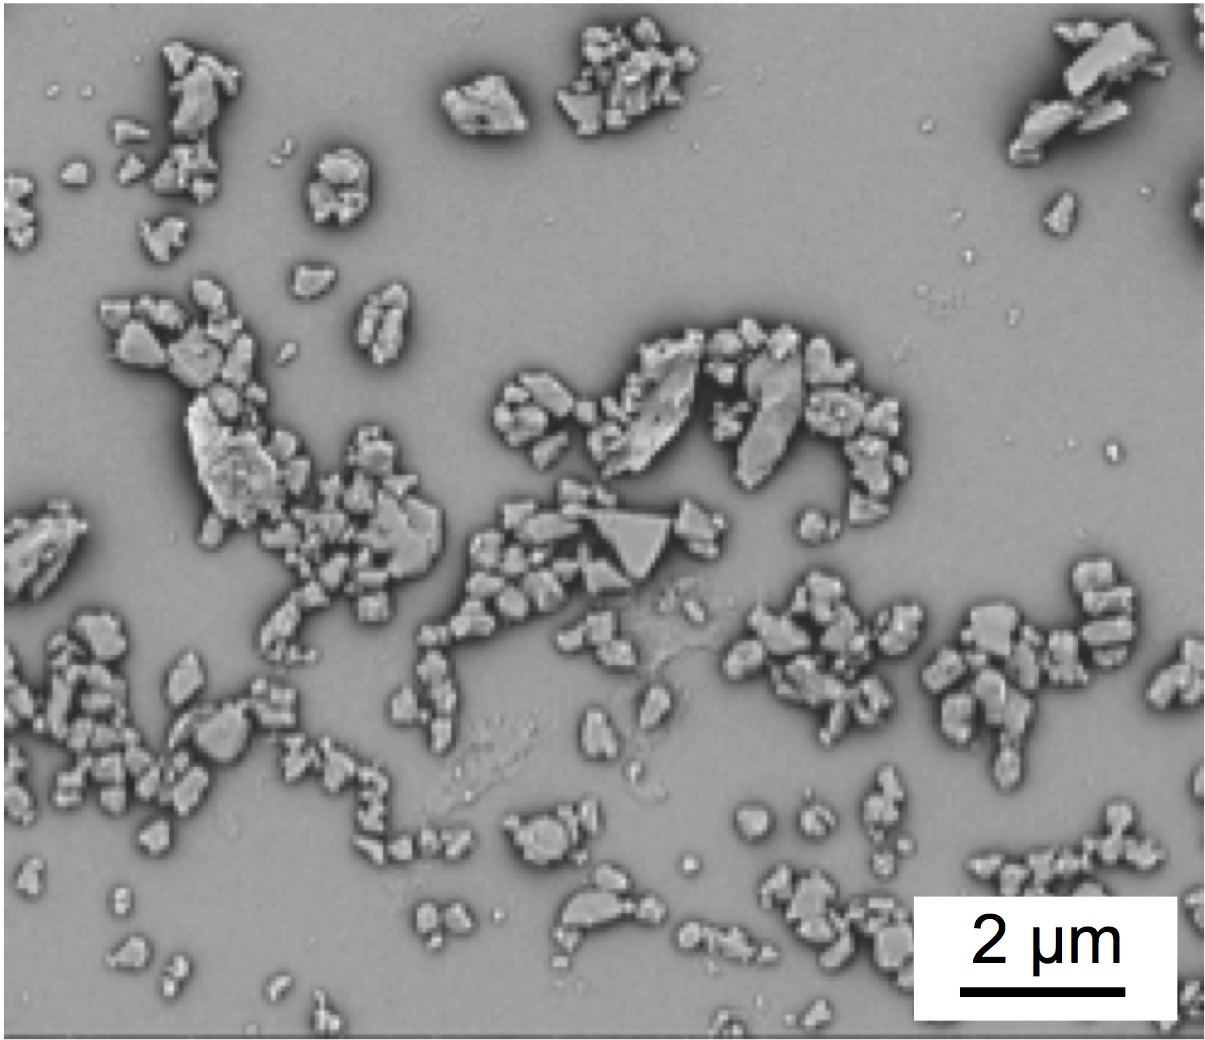
\includegraphics{Chapter-3/Figures/Figure1.png}
	\caption{SEM image of 380 ppm MgO-doped Bayer alumina powder used in this work.}
	\label{Ch3-figure:Figure1}
\end{figure}
%%%

\newpage
%%%
\begin{figure}[H]
	\centering
	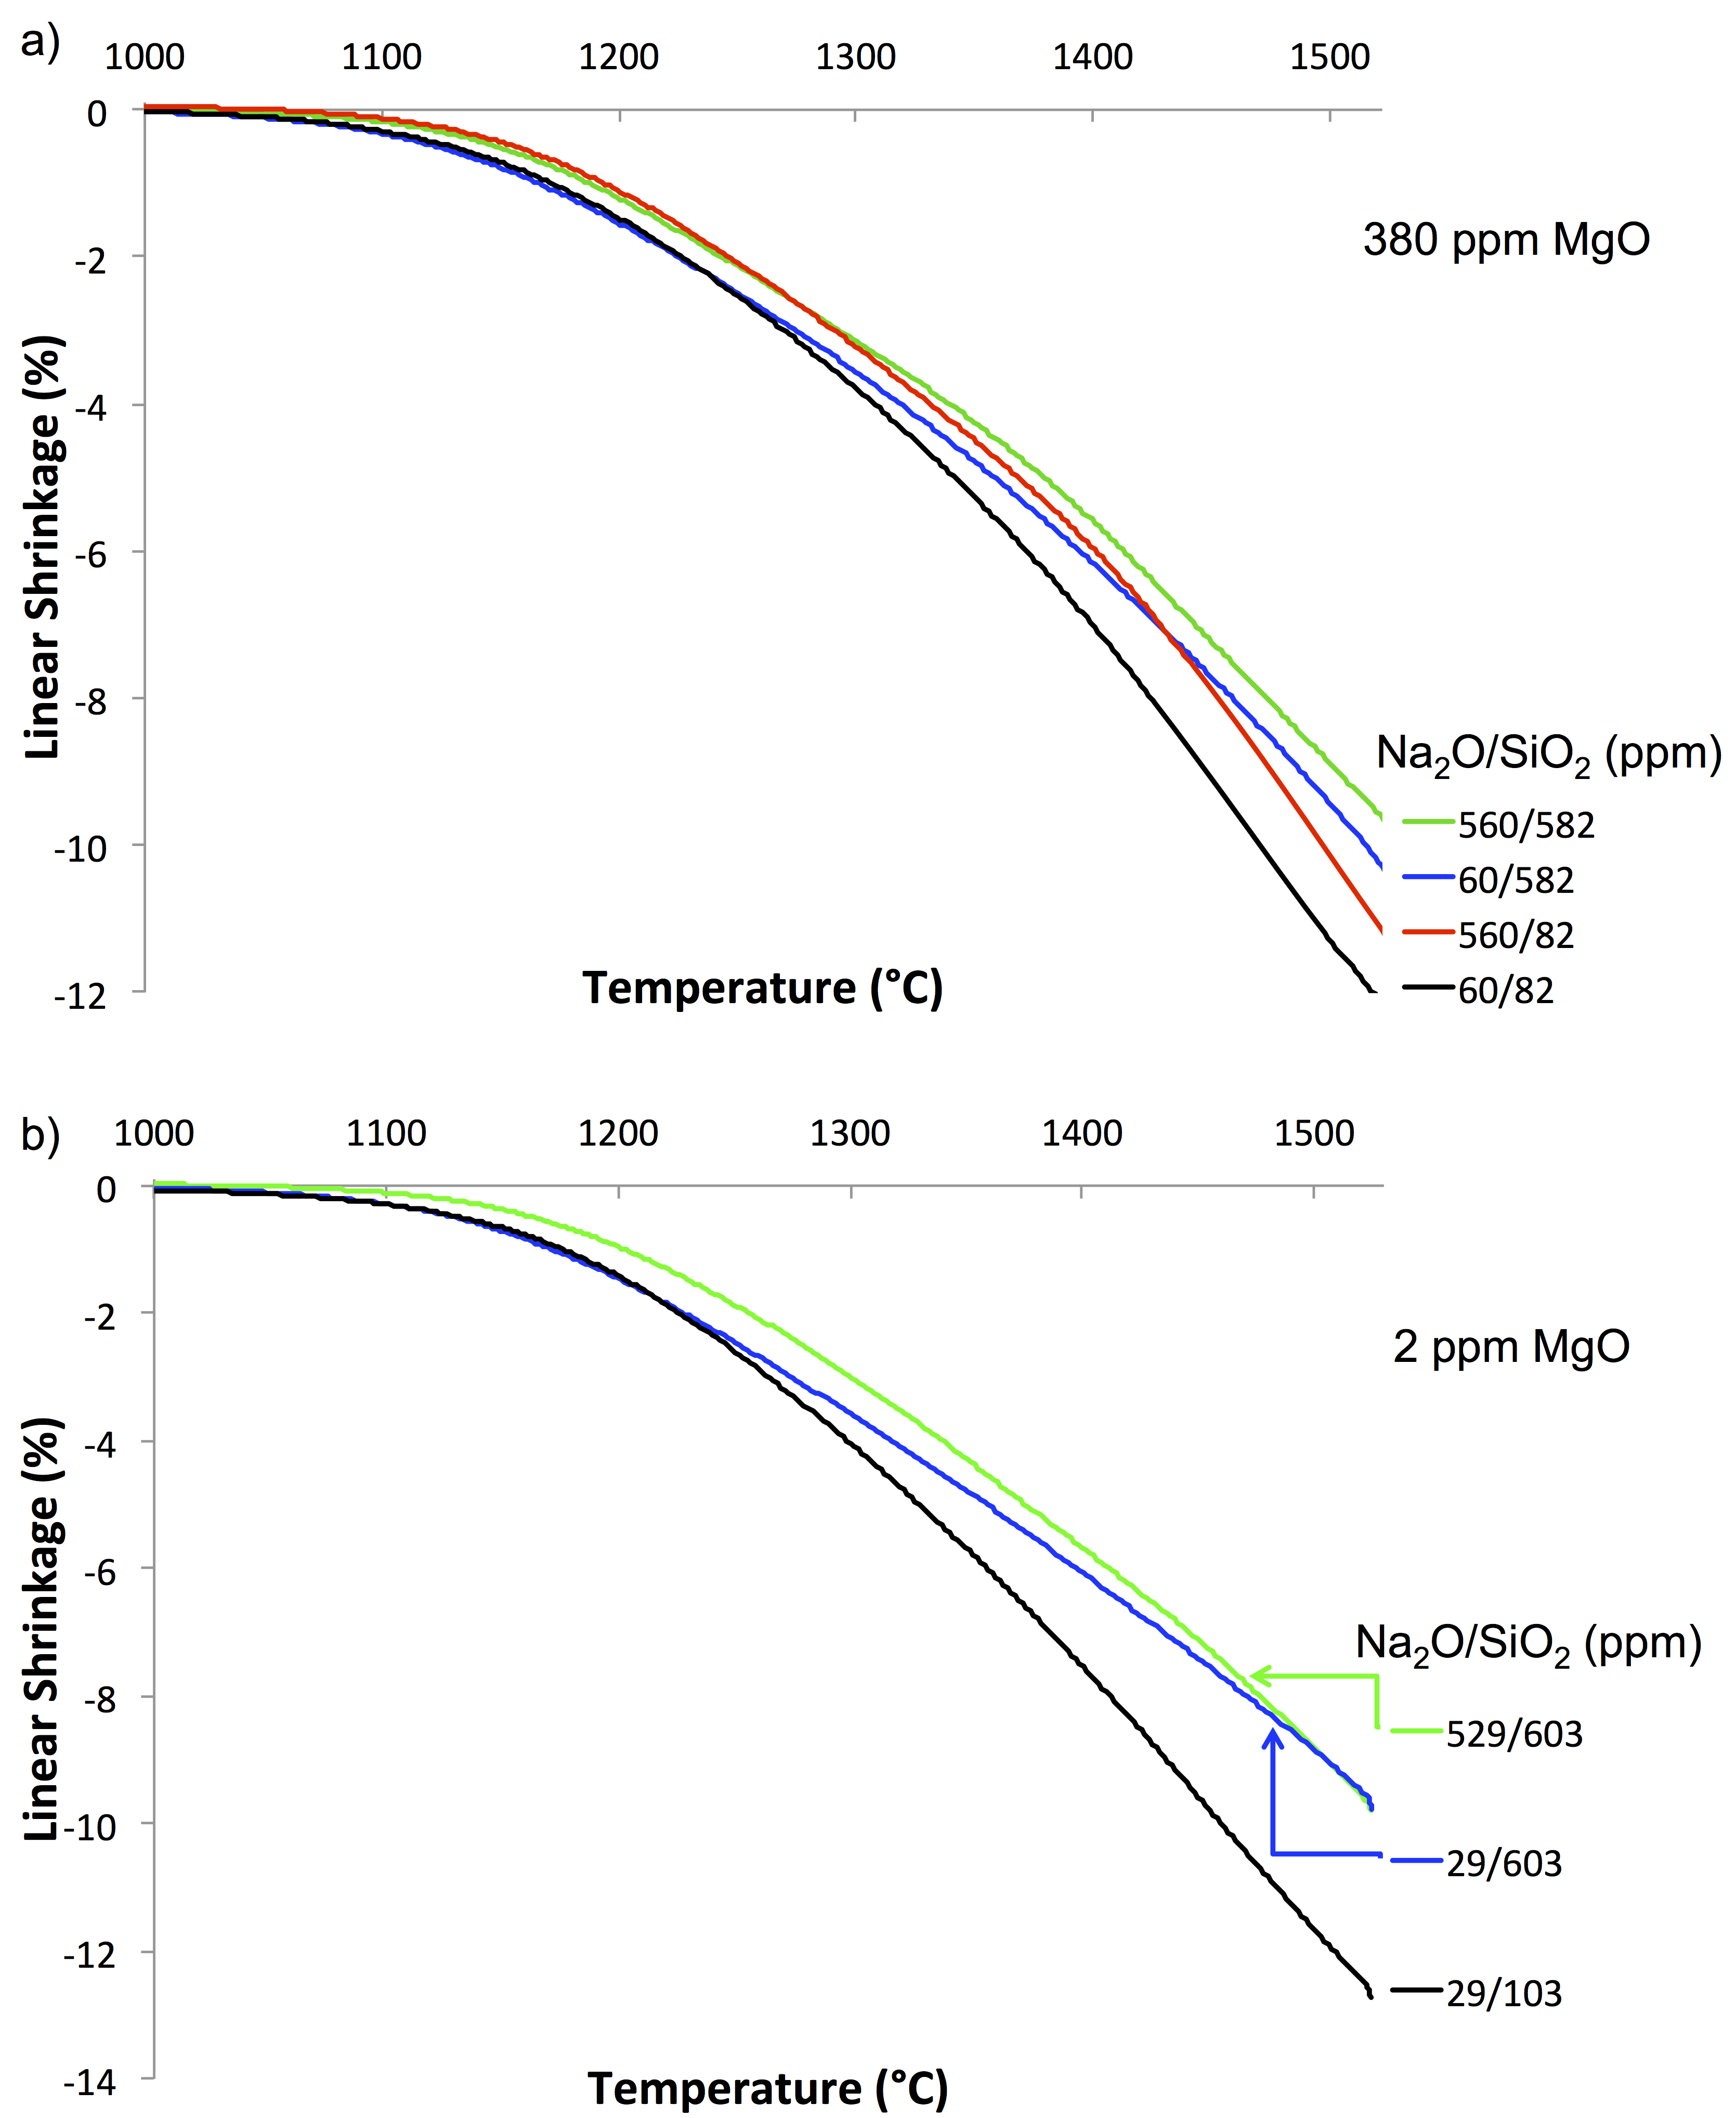
\includegraphics[width=\textwidth]{Chapter-3/Figures/Figure2.png}
	\caption{Dilatometer curves of a) 380 ppm MgO-doped and b) MgO-free \cite{Frueh2016a} Bayer alumina samples with different Na$_{2}$O/SiO$_{2}$ levels heated at 10$^{\circ}$C/min to 1525$^{\circ}$C.}
	\label{Ch3-figure:Figure2}
\end{figure}
%%%

\newpage
%%%
\begin{figure}[H]
	\centering
	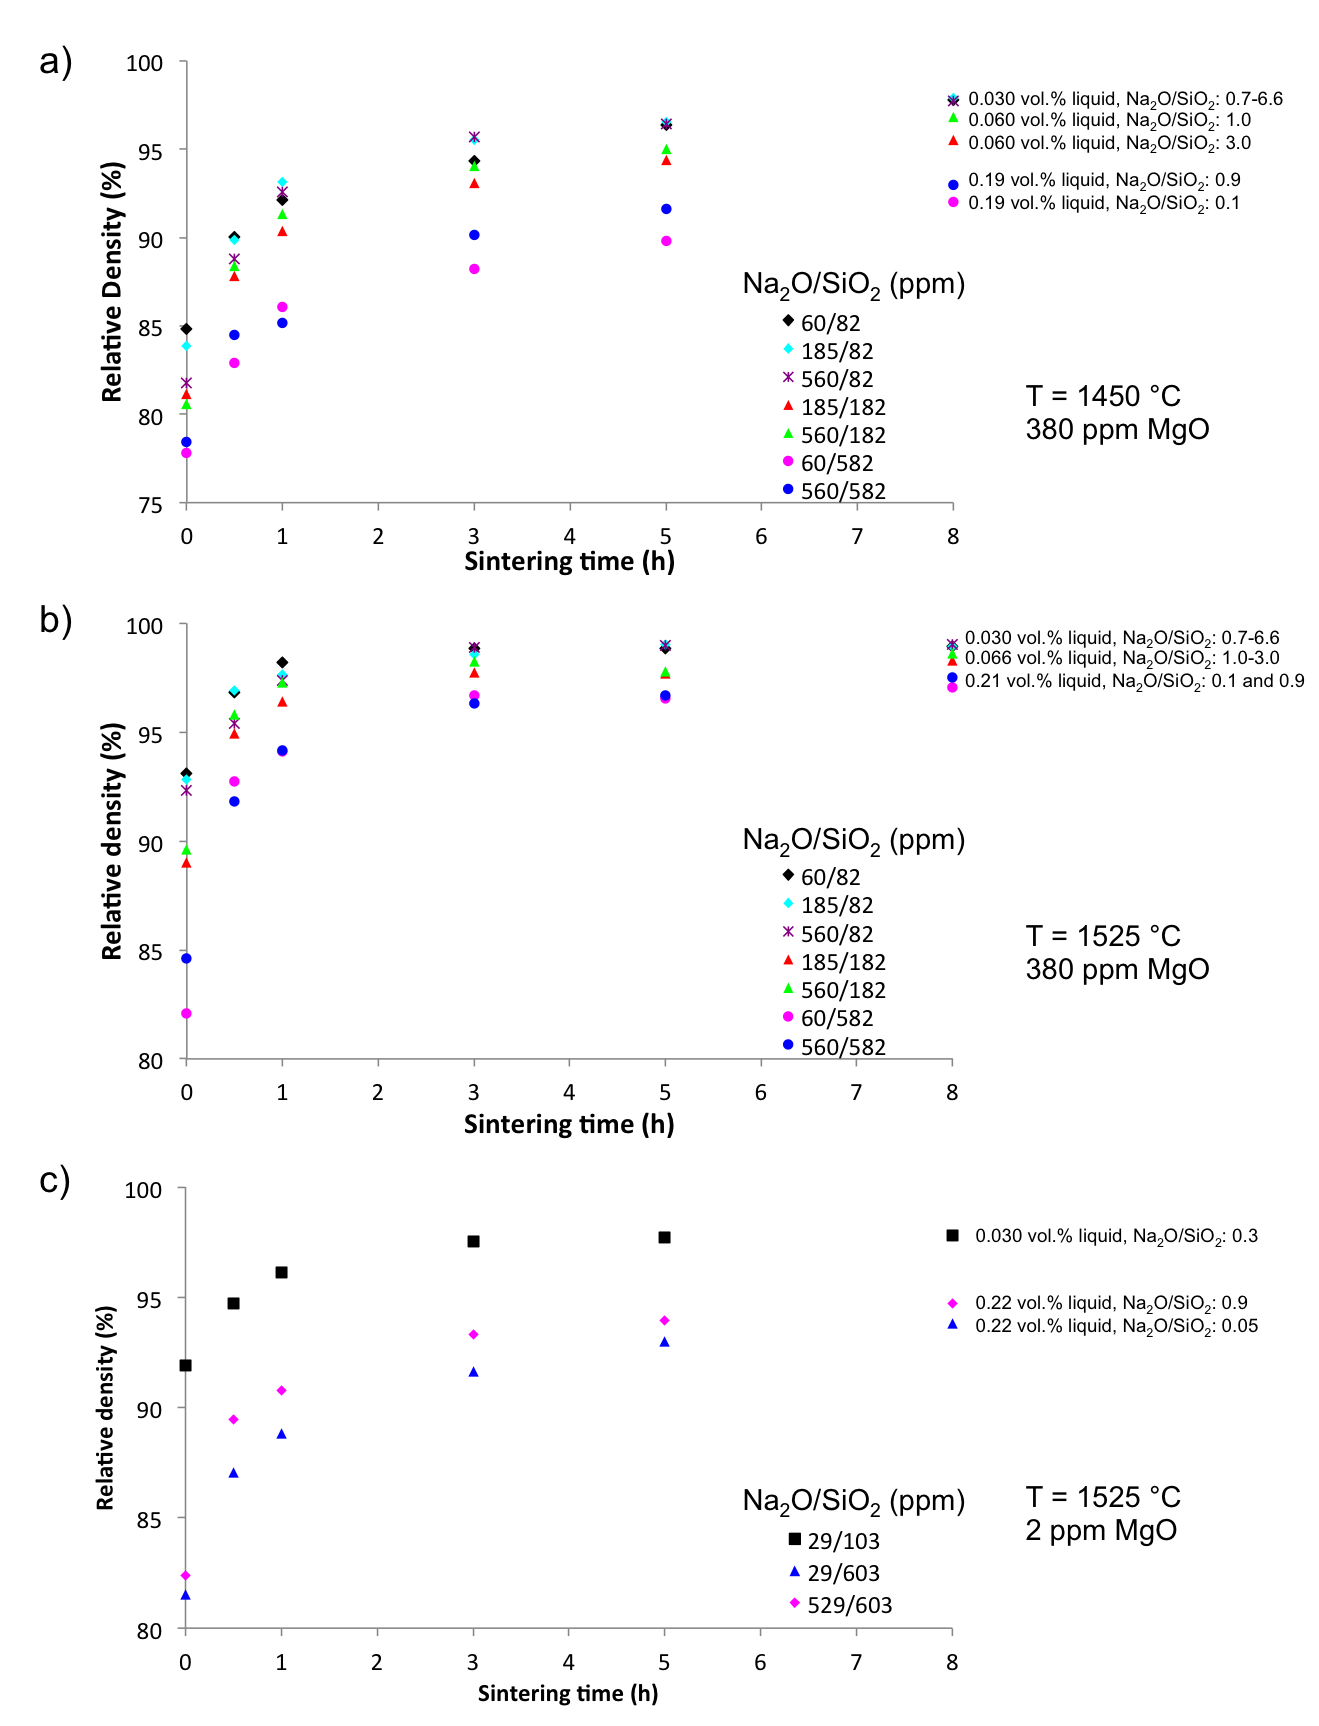
\includegraphics[width=\textwidth]{Chapter-3/Figures/Figure3.png}
	\caption{Densification kinetics of Bayer processed alumina containing different amounts Na$_{2}$O and SiO$_{2}$ and a) 380 ppm MgO sintered at 1450$^{\circ}$C, b) 380 ppm MgO sintered at 1525$^{\circ}$C, and c) 2 ppm MgO sintered at 1525$^{\circ}$C \cite{Frueh2016a}.}
	\label{Ch3-figure:Figure3}
\end{figure}
%%%

\newpage
%%%
\begin{figure}[H]
	\centering
	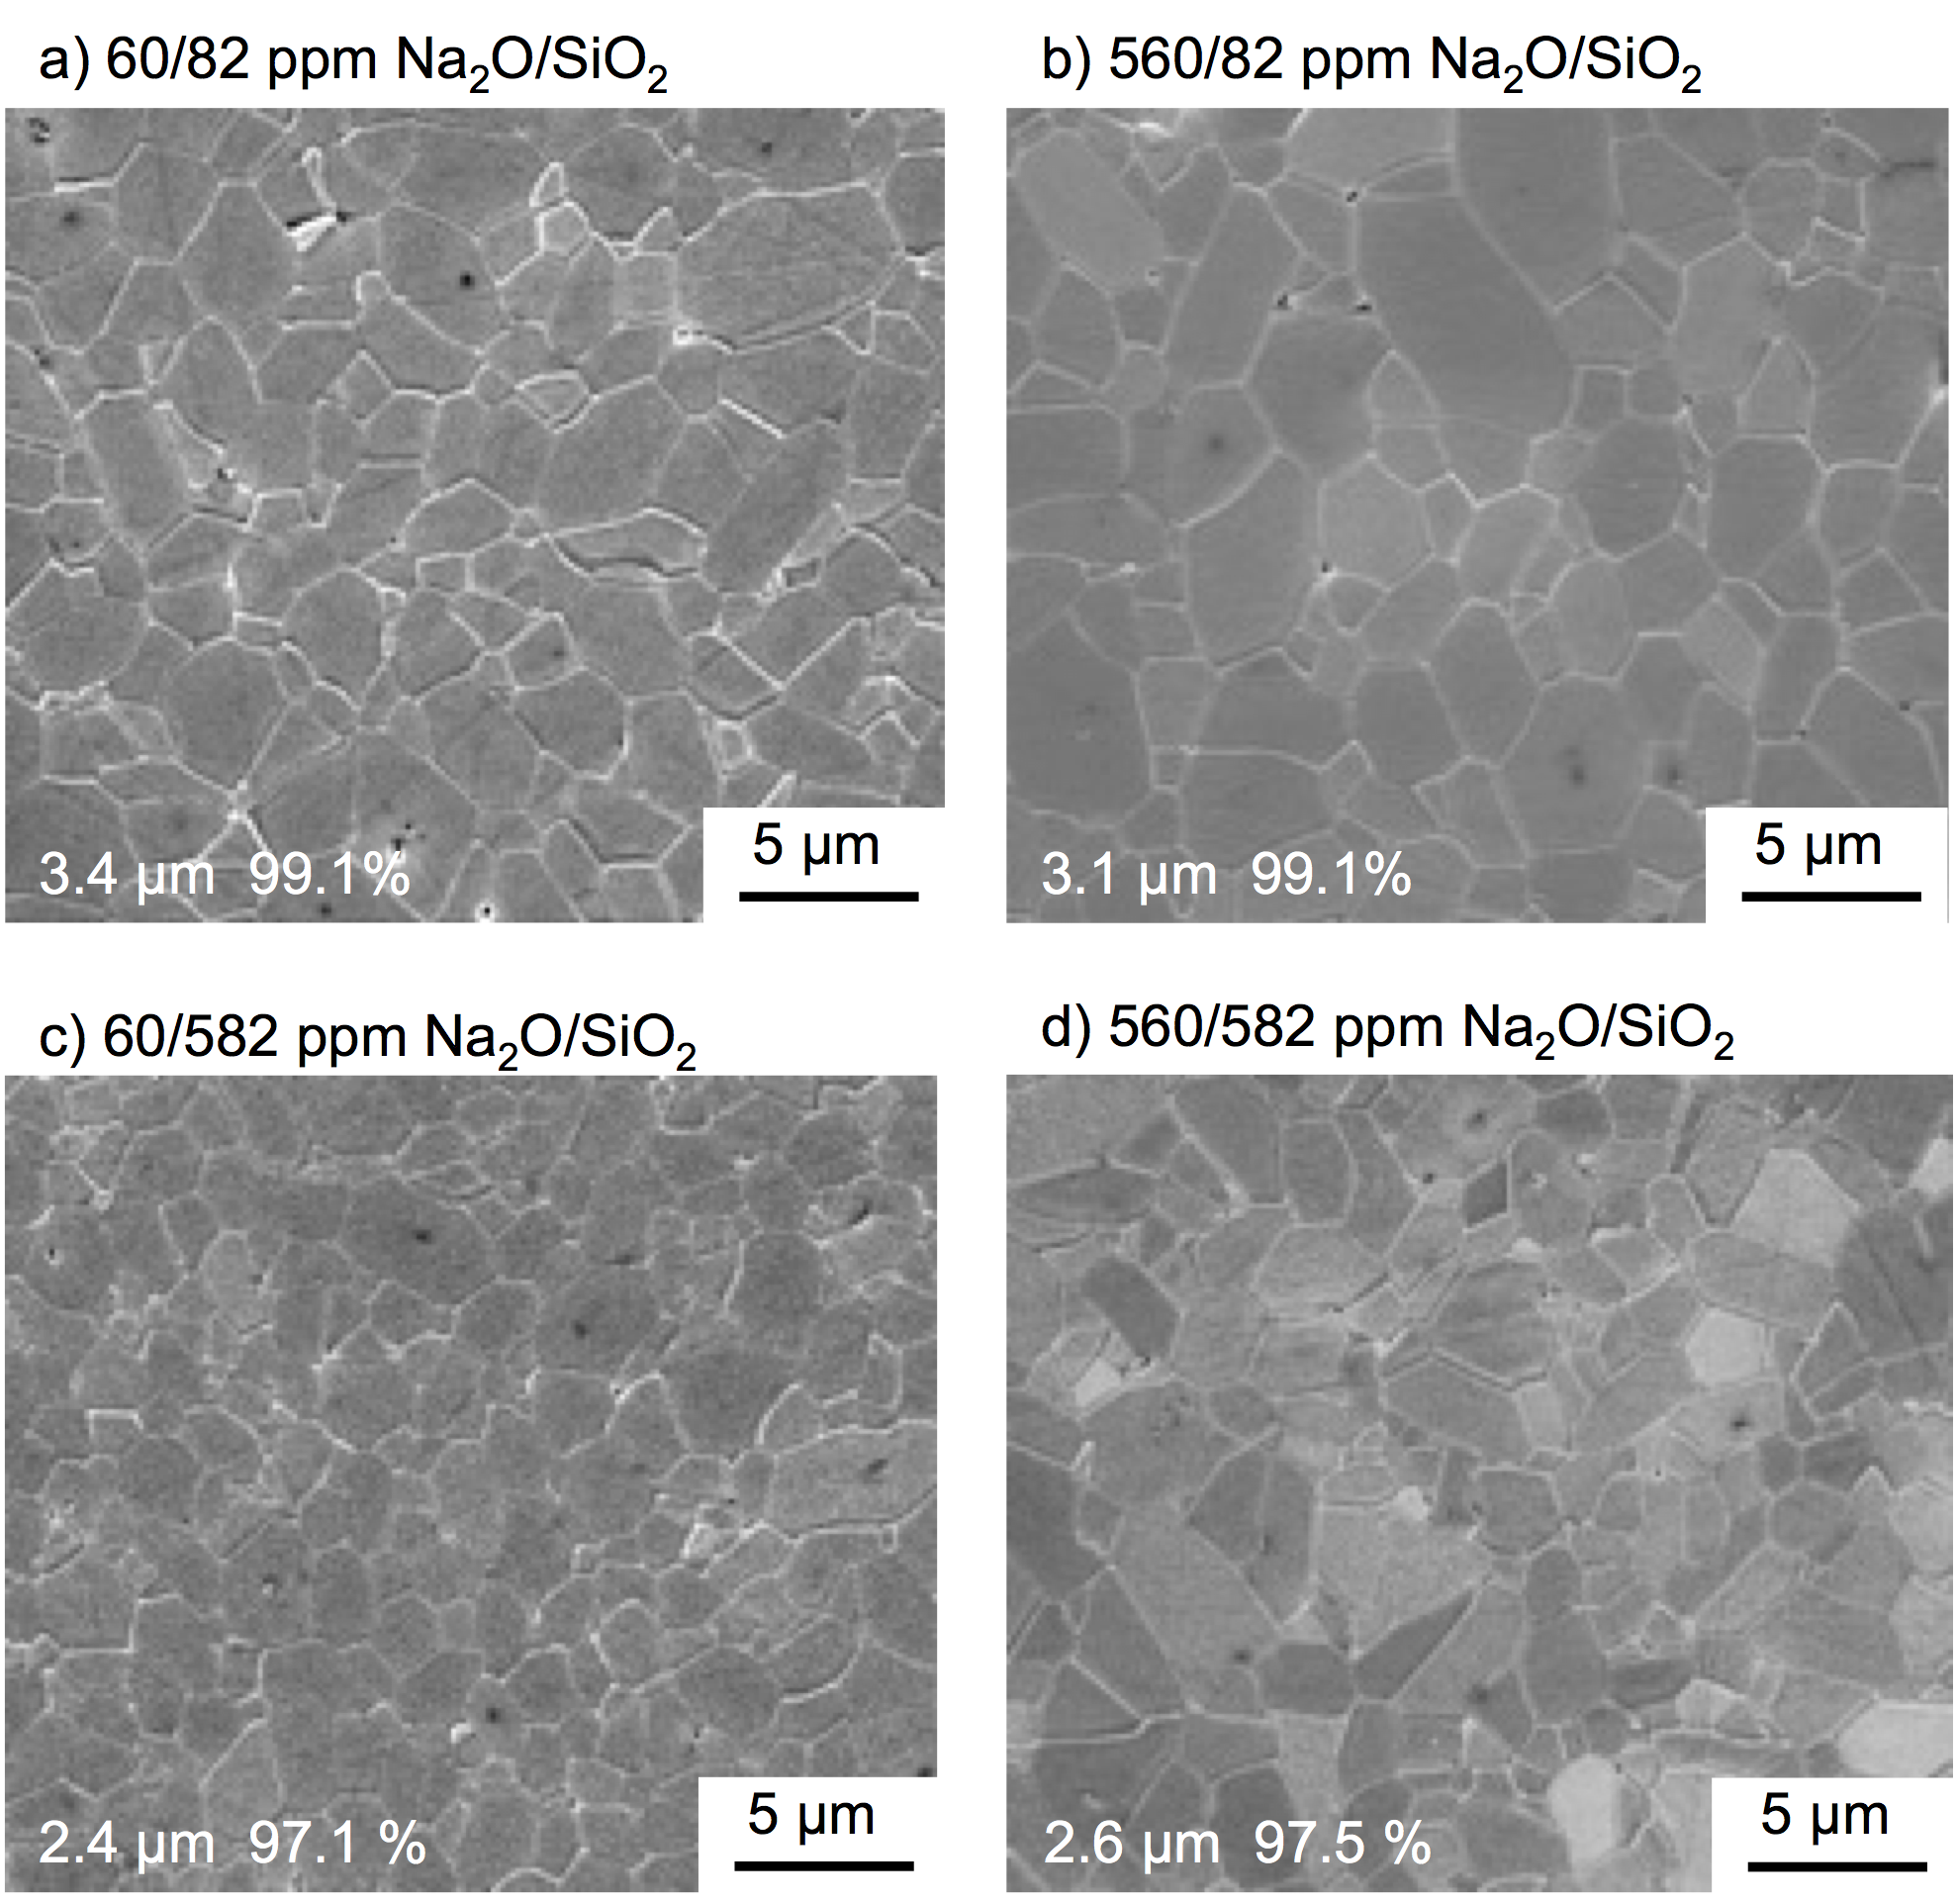
\includegraphics[width=\textwidth]{Chapter-3/Figures/Figure4.png}
	\caption{Microstructures of 380 ppm MgO-doped Bayer alumina samples with different Na$_{2}$O and SiO$_{2}$ concentrations sintered at 1525$^{\circ}$C for 8 h.}
	\label{Ch3-figure:Figure4}
\end{figure}
%%%

\newpage
%%%
\begin{figure}[H]
	\centering
	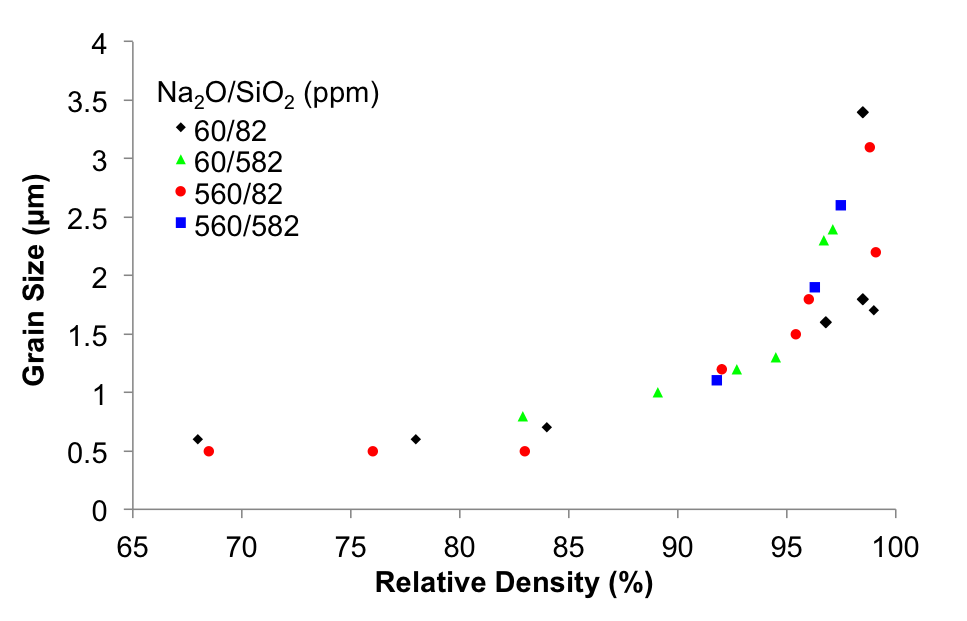
\includegraphics[width=\textwidth]{Chapter-3/Figures/Figure5.png}
	\caption{Sintering trajectories (grain size vs. relative density) for 380 ppm MgO-doped Bayer alumina samples with different Na$_{2}$O and SiO$_{2}$ concentrations.}
	\label{Ch3-figure:Figure5}
\end{figure}
%%%

\newpage
%%%
\begin{figure}[H]
	\centering
	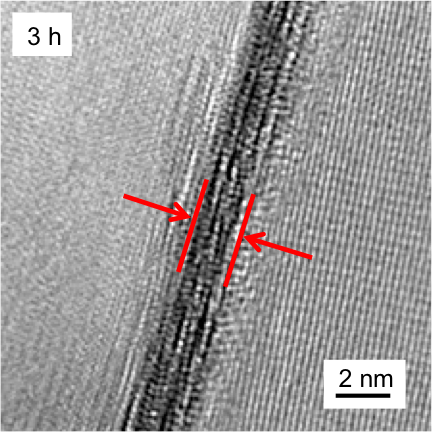
\includegraphics{Chapter-3/Figures/Figure6.png}
	\caption{Grain boundary of a sample containing 529 ppm Na$_{2}$O, 603 ppm SiO$_{2}$, and 2 ppm MgO after 3 h at 1525$^{\circ}$C.}
	\label{Ch3-figure:Figure6}
\end{figure}
%%%

\newpage
%%%
\begin{figure}[H]
	\centering
	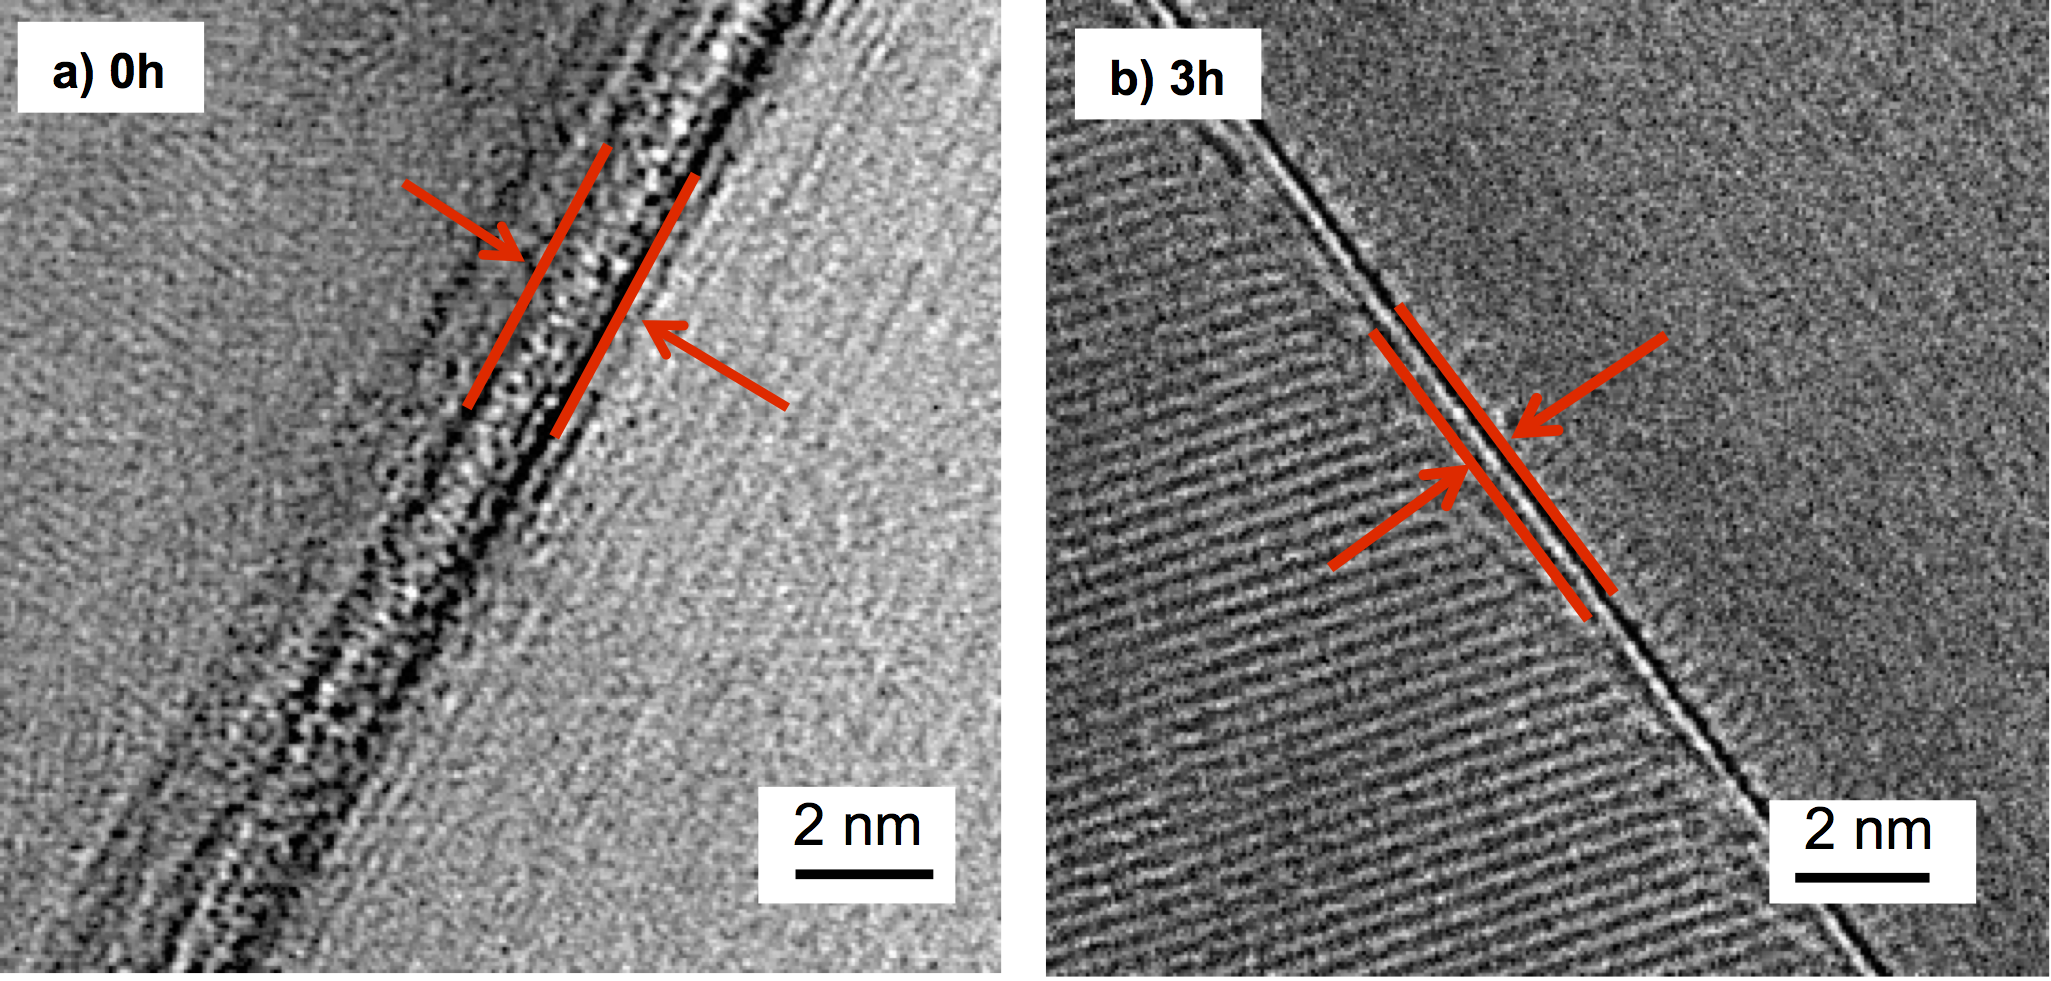
\includegraphics[width=\textwidth]{Chapter-3/Figures/Figure7.png}
	\caption{Grain boundaries of samples containing 560 ppm Na$_{2}$O, 582 ppm SiO$_{2}$, and 380 ppm MgO after a) 0 h and b) 3 h at 1525$^{\circ}$C.}
	\label{Ch3-figure:Figure7}
\end{figure}
%%%

\newpage
%%%
\begin{figure}[H]
	\centering
	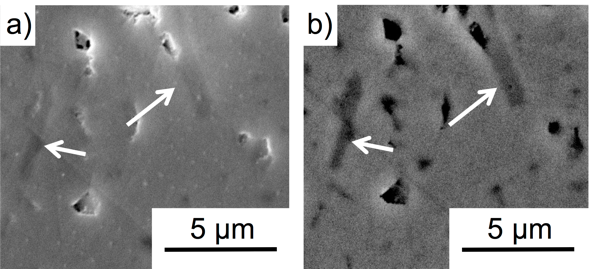
\includegraphics[width=\textwidth]{Chapter-3/Figures/Figure8.png}
	\caption{EDS of grain boundaries of samples containing 560 ppm Na$_{2}$O, 582 ppm SiO$_{2}$, and 380 ppm MgO after a) 0 h and b) 3 h at 1525$^{\circ}$C showing the Si distribution. After 0 h Si shows a stronger segregation to the grain boundaries than after 3 h.}
	\label{Ch3-figure:Figure8}
\end{figure}
%%%

\newpage
%%%
\begin{figure}[H]
	\centering
	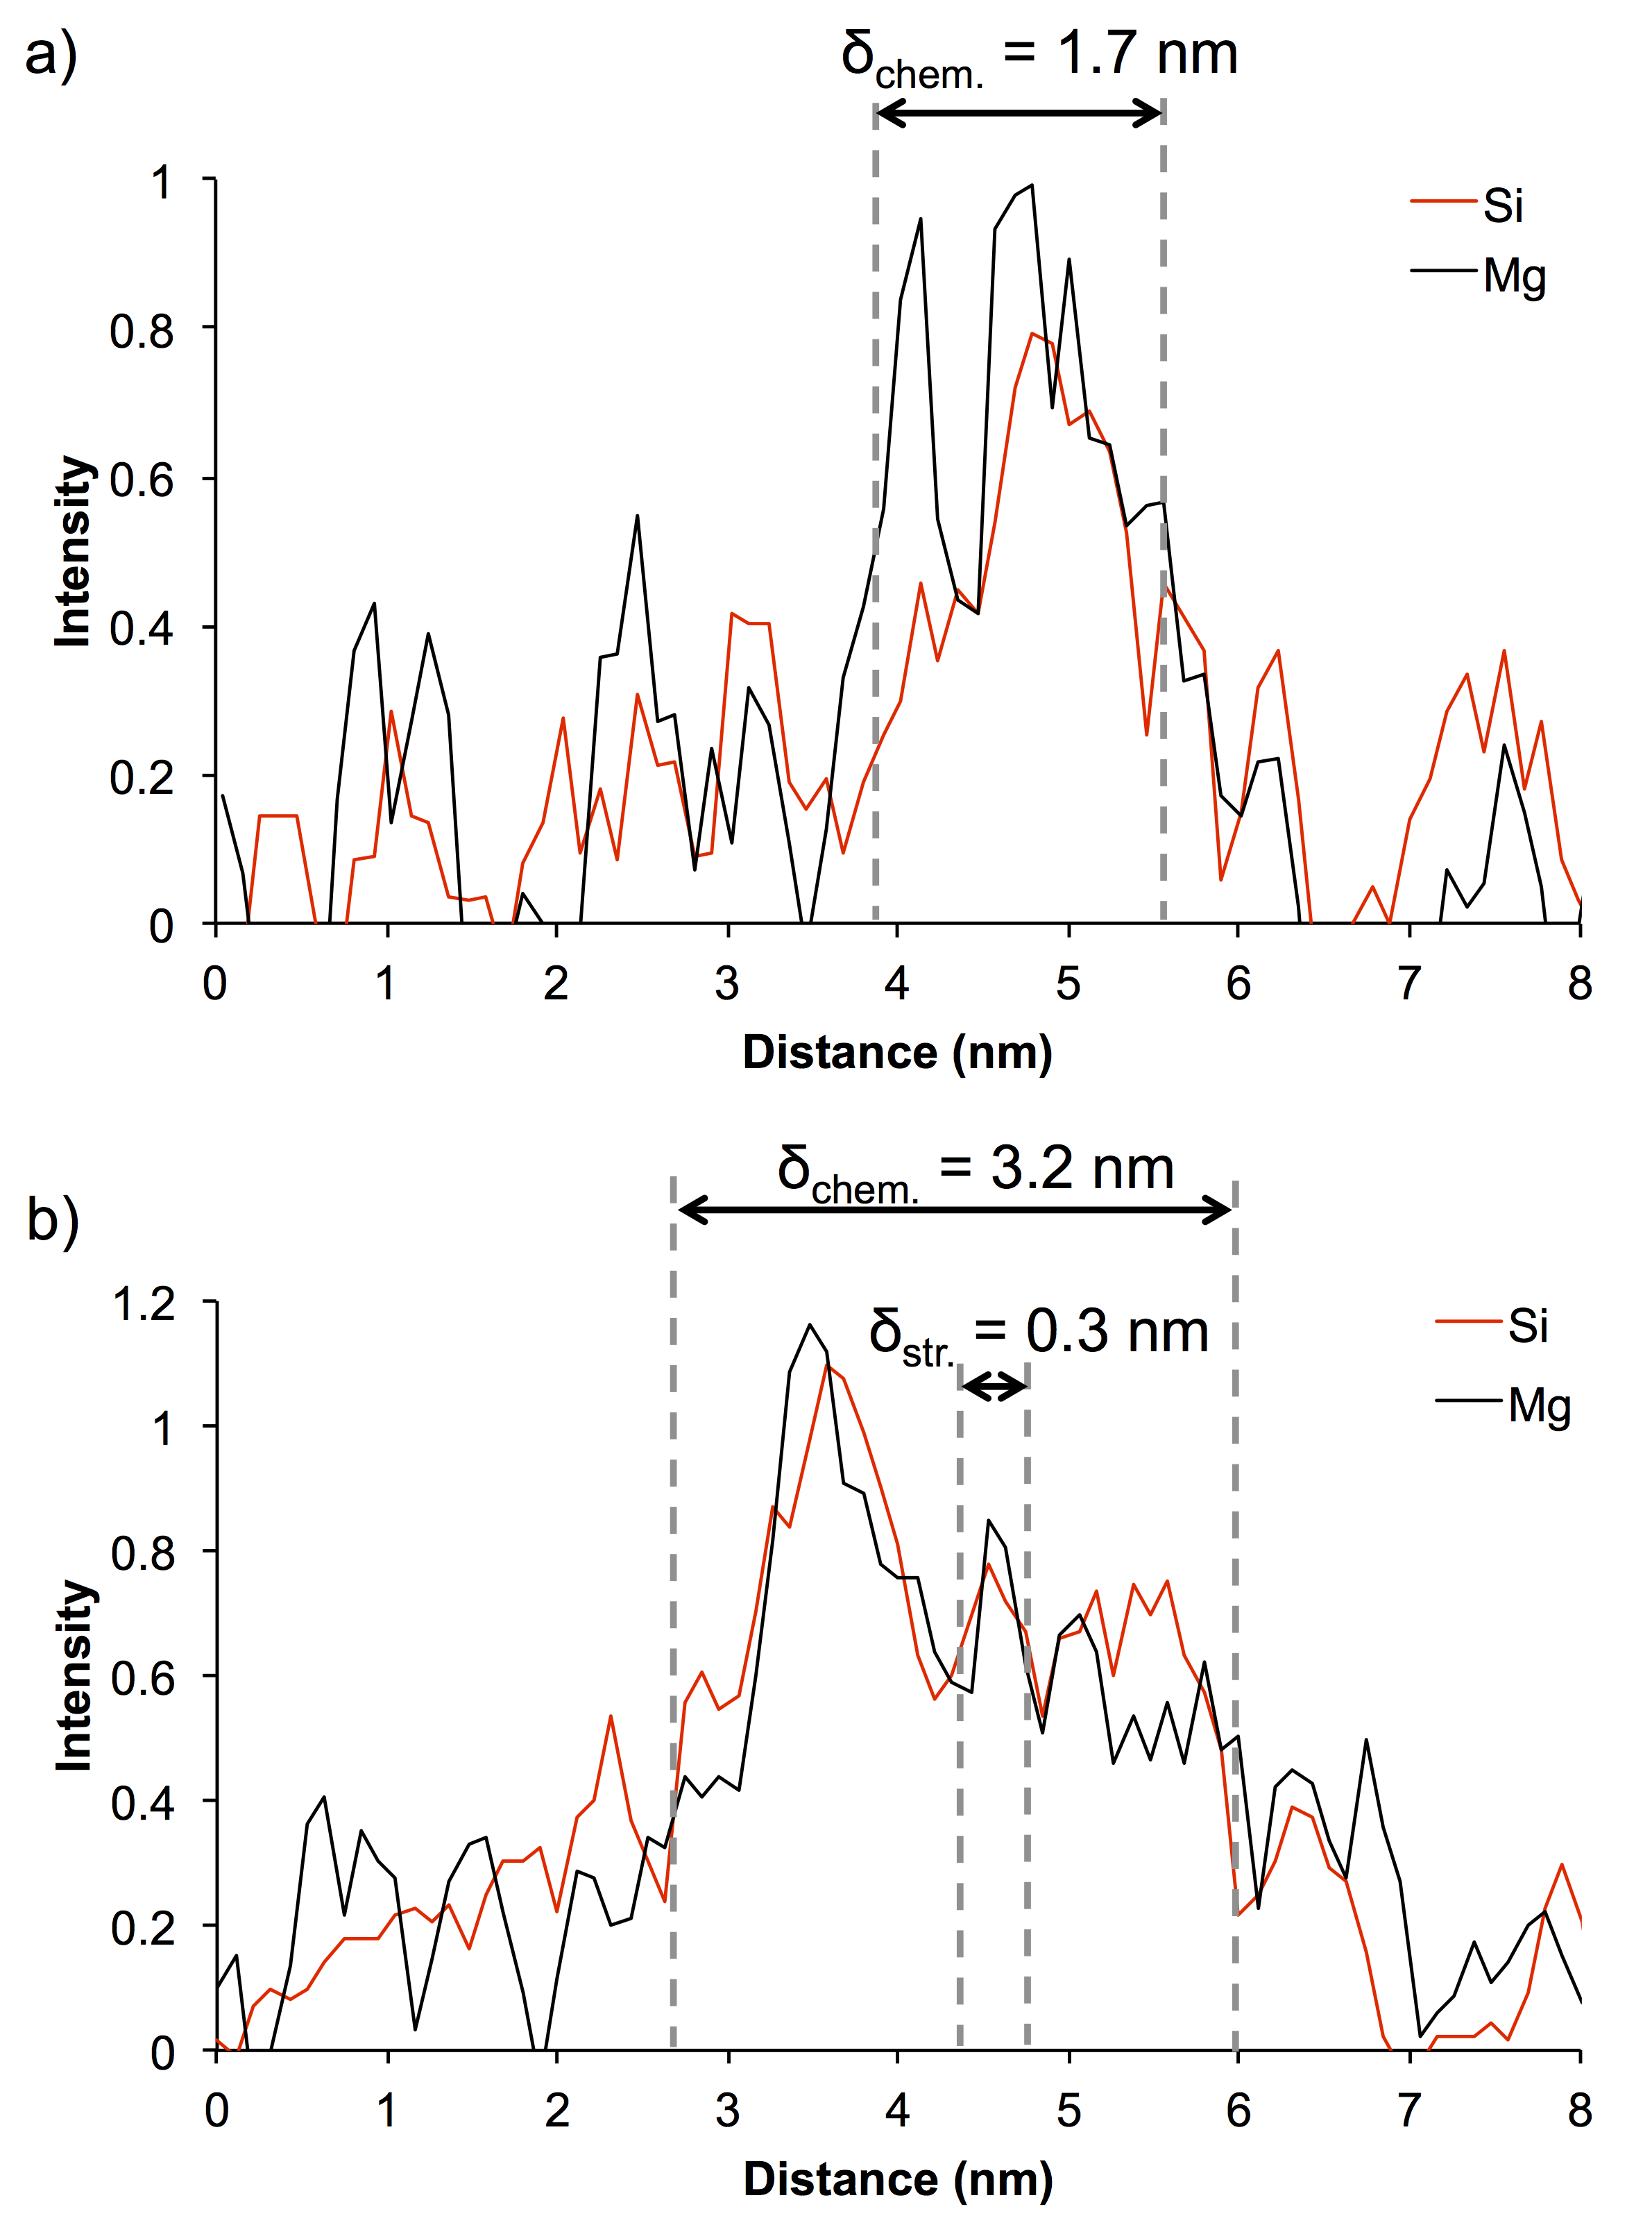
\includegraphics[width=\textwidth]{Chapter-3/Figures/Figure9.png}
	\caption{EDS line scan across a grain boundary of a sample containing 560 ppm Na$_{2}$O, 582 ppm SiO$_{2}$, and 380 ppm MgO after sintering at 1525$^{\circ}$C for a) 0 h and b) 3 h.}
	\label{Ch3-figure:Figure9}
\end{figure}
%%%

\newpage
%%%
\begin{figure}[H]
	\centering
	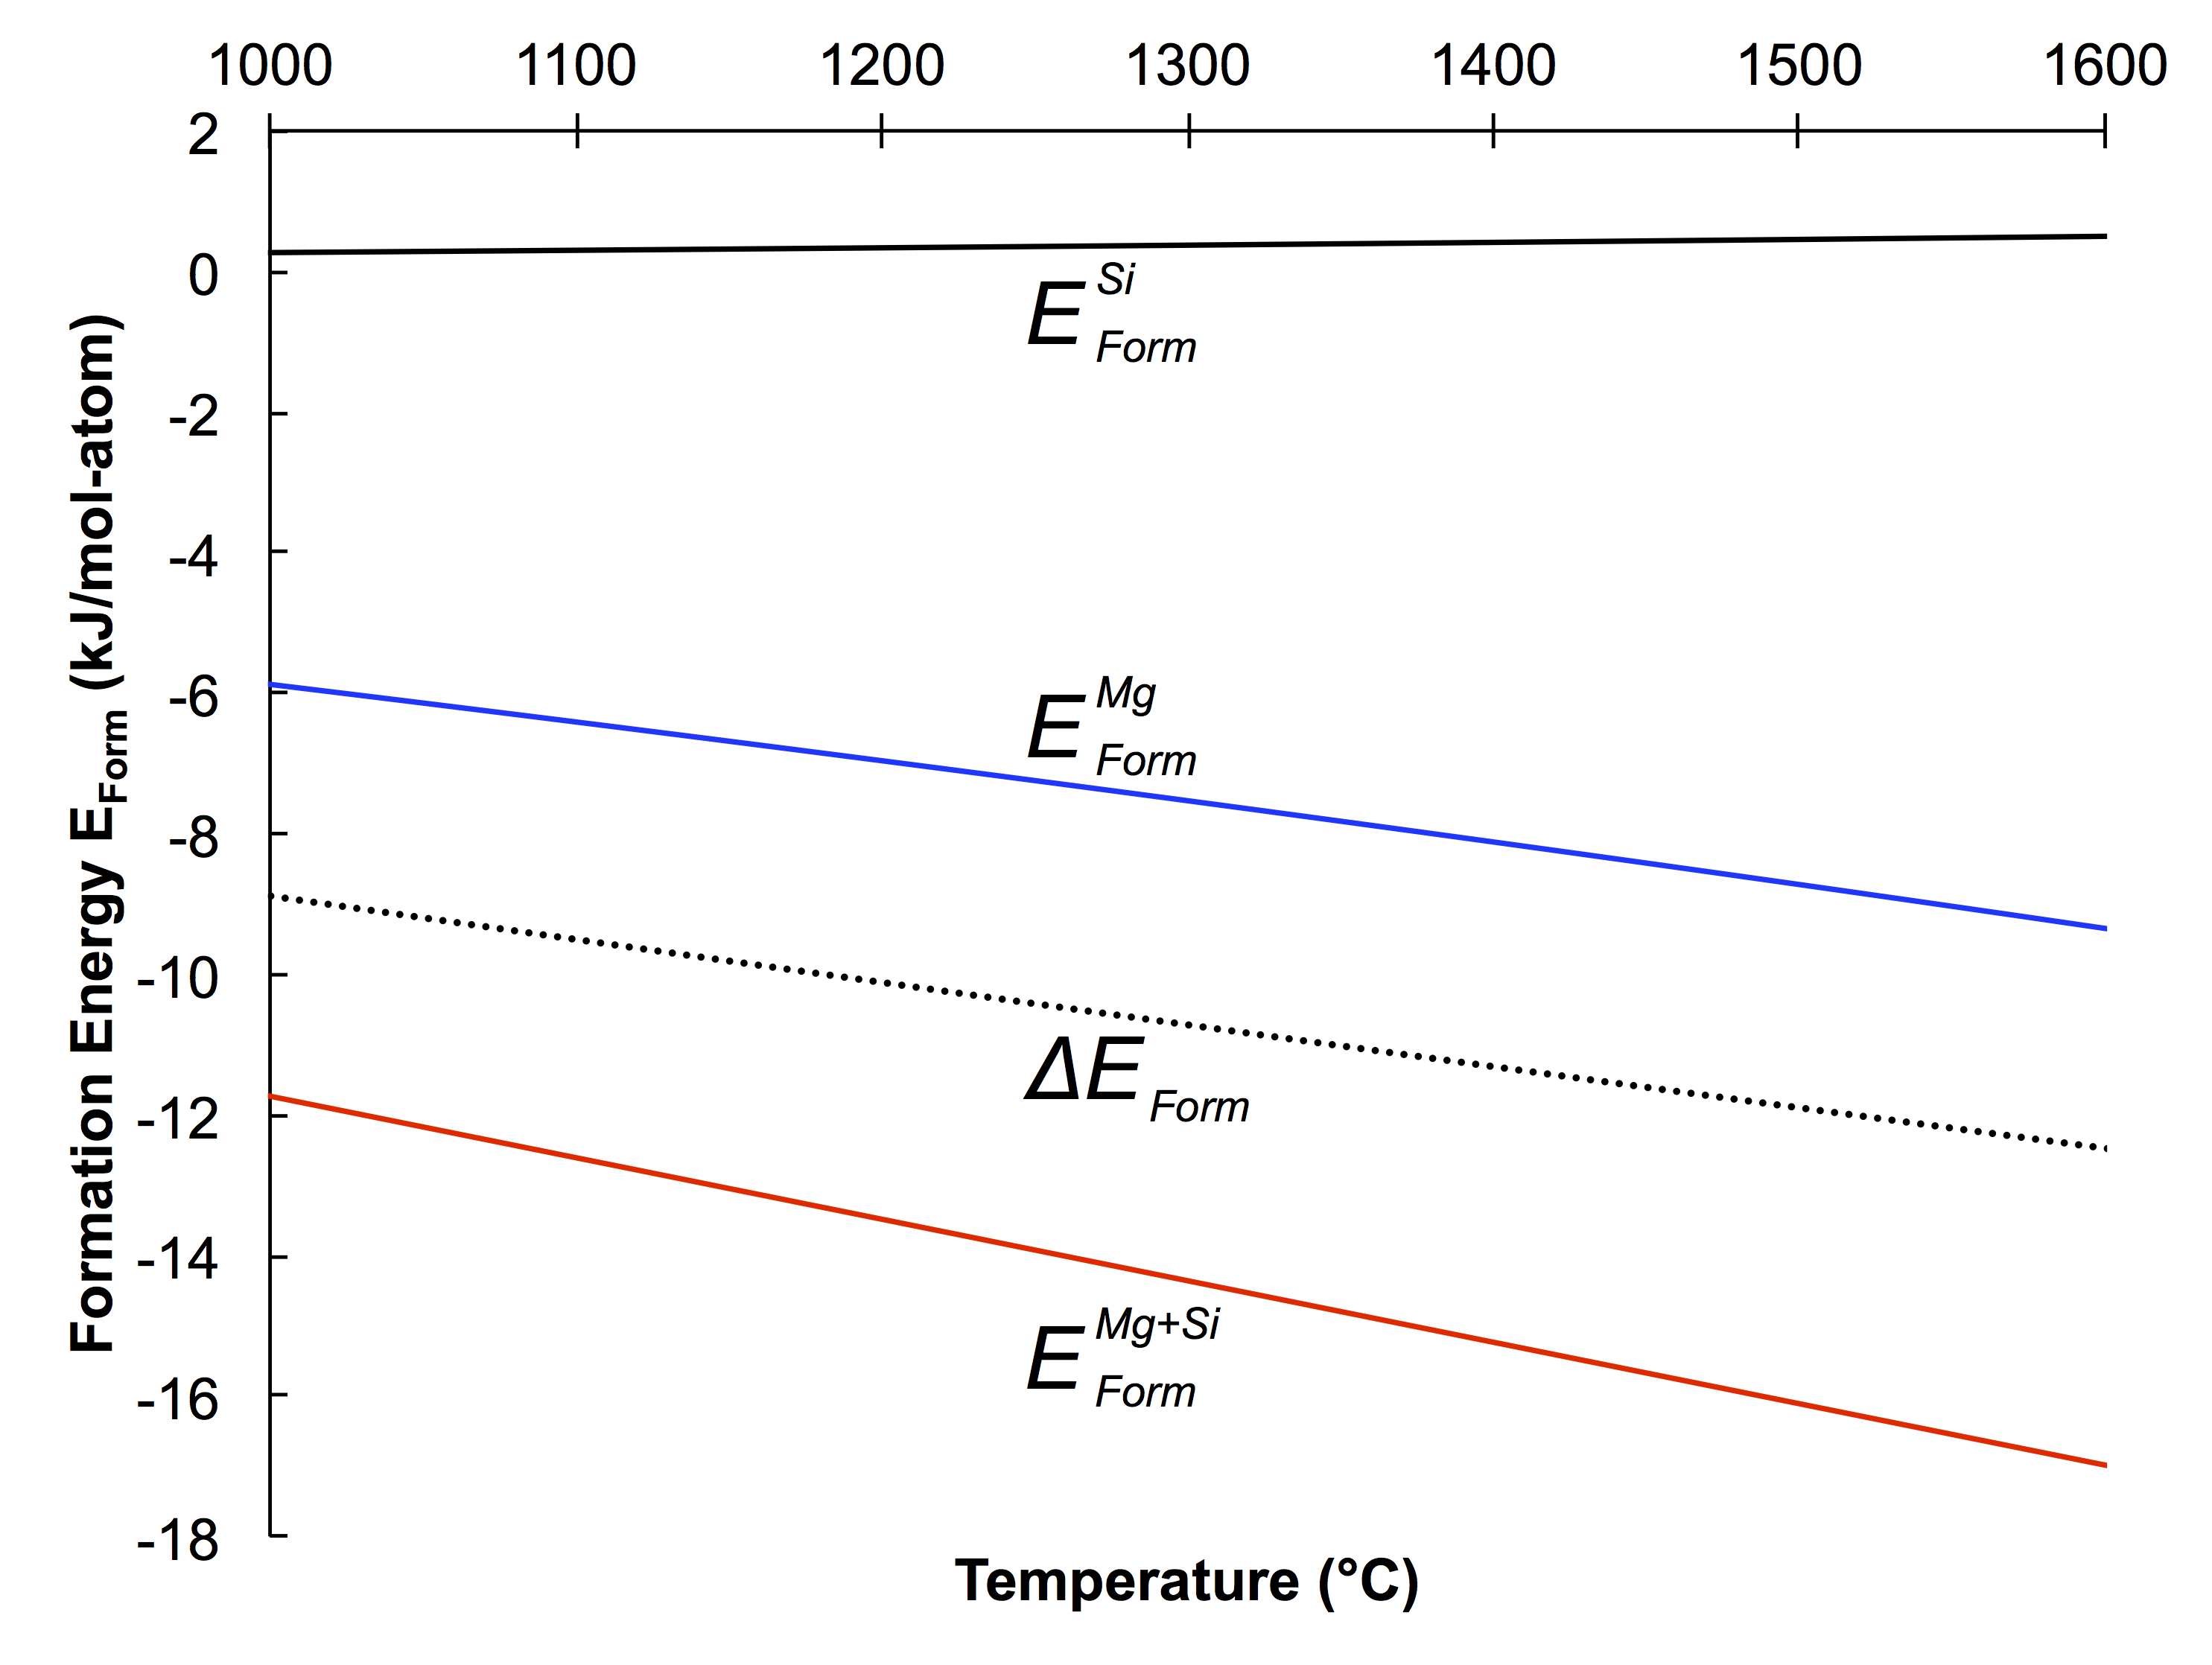
\includegraphics[width=\textwidth]{Chapter-3/Figures/Figure10.png}
	\caption{Comparison of the formation energy of $\alpha$-Al$_{2}$O$_{3}$ with an Mg-cluster ($E_{Form}^{Mg}$), Si-cluster ($E_{Form}^{Si}$) and Mg+Si-cluster ($E_{Form}^{Mg+Si}$) as a function of temperature. The formation energy difference ($\bigtriangleup E_{Form}$) between the structures was calculated from Eq. \ref{Ch3-eq: eform} to compare the formation energy values and show that it is energetically favorable to form Mg+Si-clusters over Si-clusters and Mg-clusters.}
	\label{Ch3-figure:Figure10}
\end{figure}
%%%

\newpage
%%%
\begin{figure}[H]
	\centering
	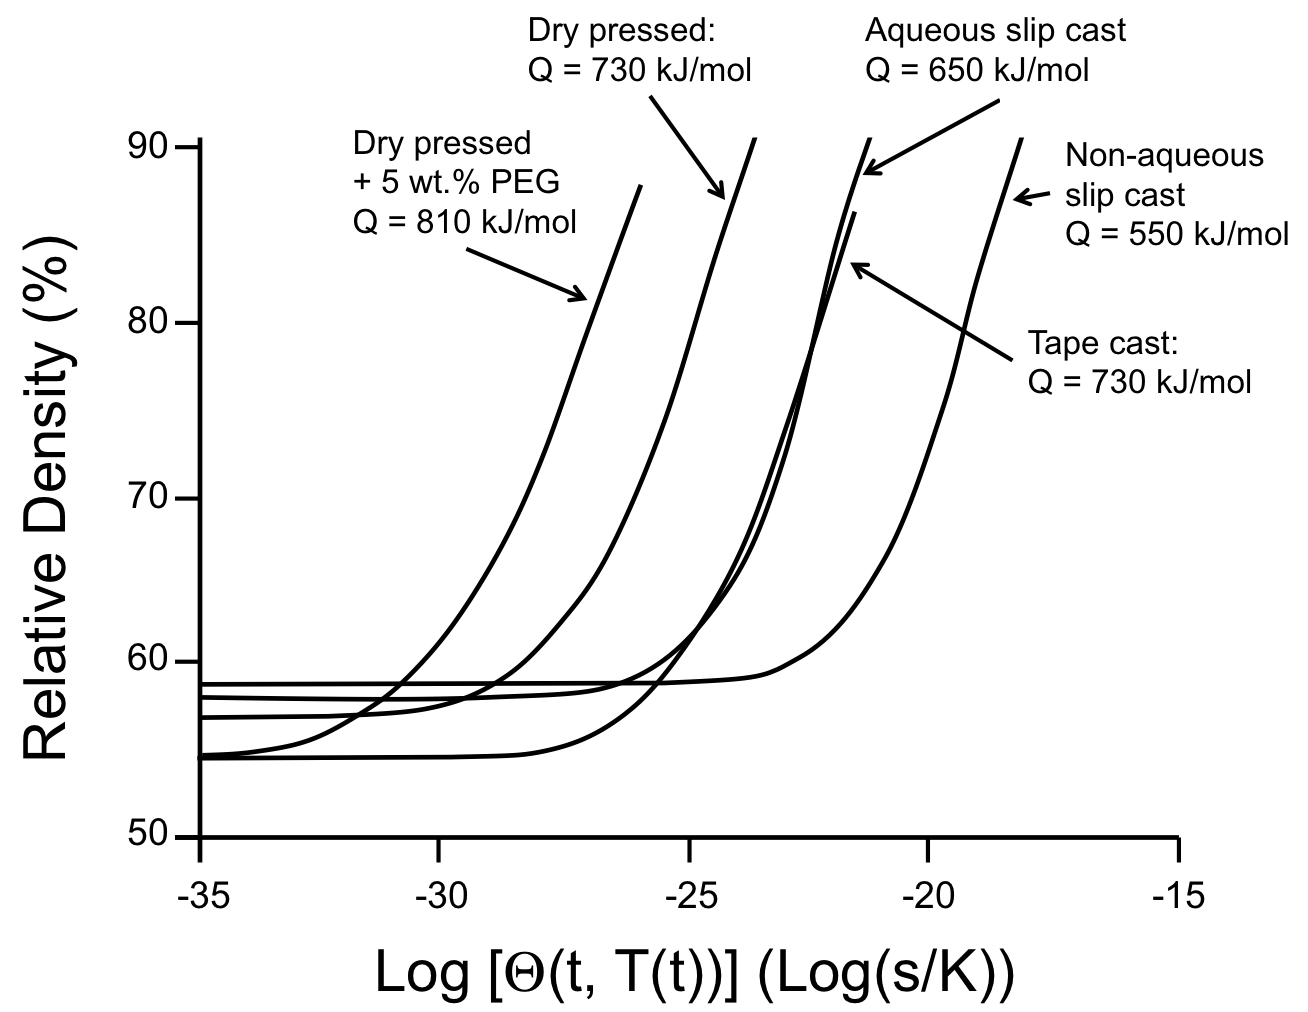
\includegraphics[width=\textwidth]{Chapter-3/Figures/Figure11.png}
	\caption{EDS maps of different oxides in 380 ppm MgO-doped Bayer alumina samples after sintering at 1525$^{\circ}$C for a-d) 0 h and e-h) 3 h. a) and e)  show the distribution of Mg, b) and f) show the distribution of Fe, c) and g) show the distribution of Na, and d) and h) show the distribution of Ca.}
	\label{Ch3-figure:Figure11}
\end{figure}
%%%

\newpage
%%%
\begin{figure}[H]
	\centering
	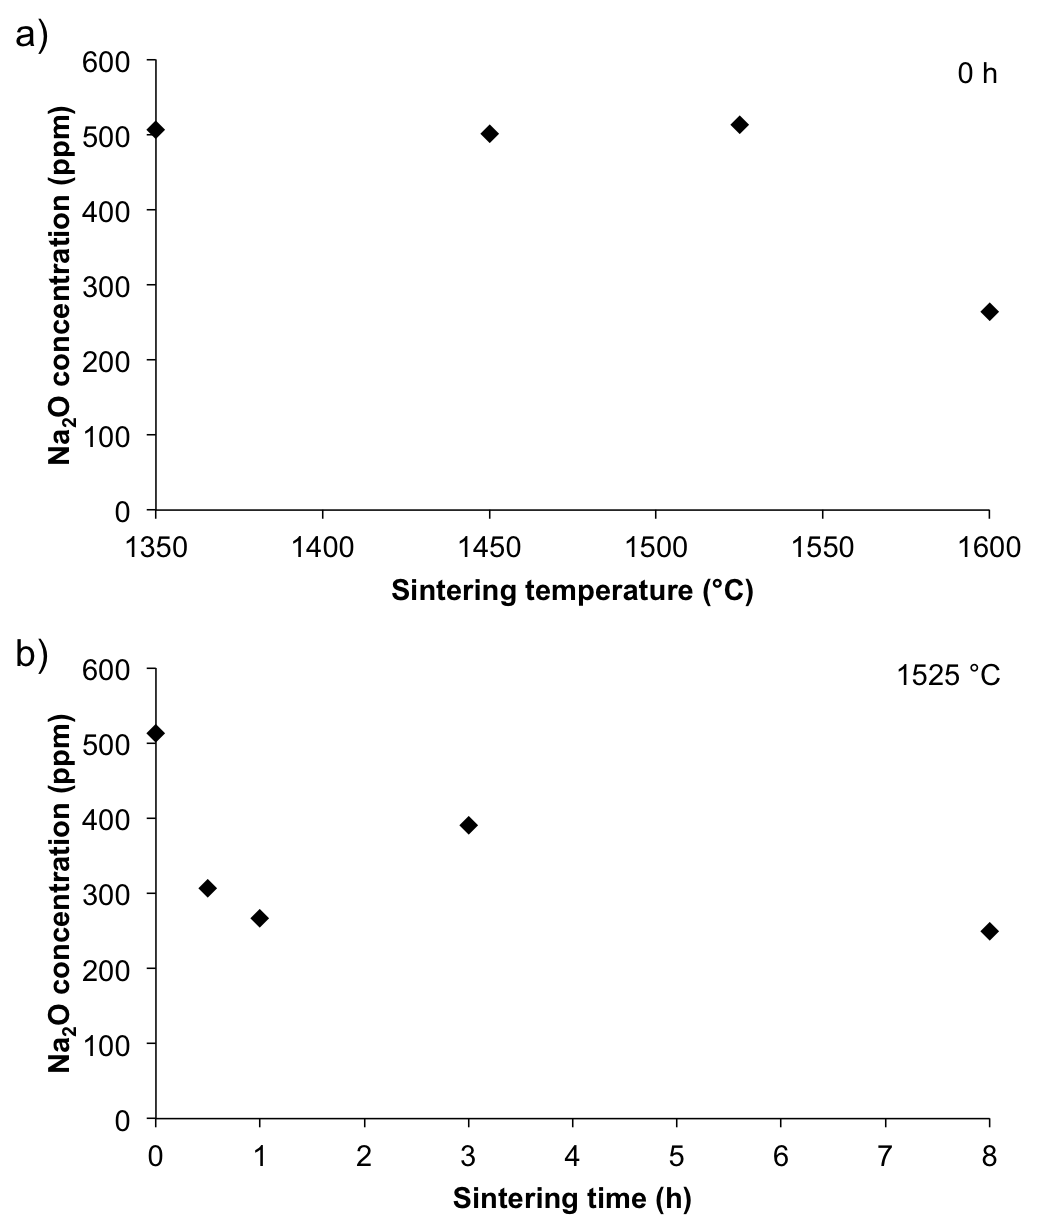
\includegraphics[width=\textwidth]{Chapter-3/Figures/Figure12.png}
	\caption{Na$_{2}$O concentration (ICP measurements) of 380 ppm MgO-doped Bayer alumina samples with 560 ppm Na$_{2}$O as a) function of sintering temperature and b) as a function of sintering time at 1525$^{\circ}$C.}
	\label{Ch3-figure:Figure12}
\end{figure}
%%%